\documentclass[11pt,letterpaper]{report}
\usepackage[utf8]{inputenc}
\usepackage[T1]{fontenc}
\usepackage{lmodern}
\usepackage[margin=1in]{geometry}
\usepackage{amsmath,amssymb,mathtools}
\usepackage{graphicx,array,longtable}
\usepackage{tikz,float}
\usetikzlibrary{arrows.meta,positioning}
\tikzset{flowbox/.style={draw,rounded corners=2pt,fill=black!3,align=center,
 text width=12cm,inner sep=6pt,font=\small},
 halfbox/.style={flowbox,text width=5.5cm},
 flowarrow/.style={-{Stealth[length=2.2mm]},thick}}

\usepackage{enumitem}
\usepackage{microtype}
\usepackage[unicode,hidelinks]{hyperref}
\newcommand{\fitmath}[1]{\begingroup\setbox0=\hbox{$\displaystyle #1$}\ifdim\wd0>\linewidth\resizebox{\linewidth}{!}{$\displaystyle #1$}\else\displaystyle #1\fi\endgroup}
\setlist{itemsep=0.3em,topsep=0.5em}
\setlength{\parindent}{0pt}
\setlength{\parskip}{0.55em}
\setlength{\emergencystretch}{3em}
\setcounter{secnumdepth}{2}
\setcounter{tocdepth}{1}
\renewcommand{\thechapter}{\arabic{chapter}}
\renewcommand{\thesection}{\arabic{section}}
\renewcommand{\thesubsection}{\thesection.\arabic{subsection}}
\title{Stochastic Marxian Macroeconomics\\[0.6em]\large A working draft on Automation, Fictitious Capital, and Networked Crises}
\author{Félix Alfonso Camacho Moya}
\date{}
\begin{document}
\maketitle
\begingroup
\small
\setlength{\parskip}{0pt}
\tableofcontents
\endgroup
\clearpage
\chapter{Microeconomic Foundations of the TRPF: Stochastic Automation, Superprofits, and Mean Field Equilibria}
\section{Introduction \& The Micro-Macro Paradox in Marx}
In classical political economy, the dynamic trajectory of capitalist accumulation is characterized by a structural contradiction between individual rationality and systemic sustainability. In \emph{Capital}, Volume III (Part III), Karl Marx articulated this contradiction as the \textbf{Tendency of the Rate of Profit to Fall (TRPF)}. The core mechanism is straightforward yet paradoxically elusive in deterministic frameworks:

\begin{enumerate}
\item Individual capitalists face competitive pressure in commodity markets where market prices gravitate around the socially necessary labor time embodied in goods.
\item To capture temporary excess earnings---\emph{surplus-profit} or \emph{superprofit} (\emph{Extra-Mehrwert})---an individual firm introduces labor-saving machinery ahead of competitors. This unilateral innovation lowers the firm's private unit cost below the general market value of the commodity.
\item However, under generalized competition, innovations diffuse across the sector. As competitors adopt the new technological baseline, the individual advantage disappears, the socially necessary labor time required to produce the commodity declines, and market prices fall.
\item Because living labor ($V$) is the sole source of surplus-value ($S$), the widespread substitution of living labor by dead constant capital ($C$) raises the systemic \textbf{organic composition of capital} ($\omega =C/V$). Unless compensated by a proportional increase in the rate of exploitation ($e=S/V$), the aggregate rate of profit across society:
\[
r=\frac{S}{C+V}=\frac{e}{\omega +1}
\]
inexorably declines.
\end{enumerate}
\subsection{Limitations of Classical Deterministic Models}
For decades, analytical formulations of this tendency were mired in the Okishio (1961) theorem debate. Nobuo Okishio demonstrated that under fixed real wages, cost-reducing innovations chosen by individual capitalists cannot depress the equilibrium rate of profit computed via standard Perron-Frobenius eigenvalues on Leontief input-output matrices.

However, the Okishio framework suffers from two structural simplifications:

\begin{itemize}
\item \textbf{Static Comparative Equilibrium:} It ignores path-dependent, out-of-equilibrium dynamics during technological transition periods, treating innovation as an instantaneous comparative-static jump rather than a continuous race under uncertainty.
\item \textbf{Absence of Real Turbulence and Moral Depreciation:} Deterministic equilibrium models abstract away asset volatility, obsolescence risk (\emph{moralischer Verschleiß}), and stochastic class struggle over wage and exploitation shares.
\end{itemize}
\subsection{The Stochastic Mean Field Game (MFG) Synthesis}
To rigorously formalize Marx's micro-macro paradox, this paper operationalizes the accumulation process using the mathematics of \textbf{Stochastic Optimal Control} and \textbf{Mean Field Games (MFG)} (Lasry \& Lions, 2007; Huang, Malhamé, \& Caines, 2006).

Within this framework:

\begin{itemize}
\item The individual firm solves a stochastic Hamilton-Jacobi-Bellman (HJB) problem, choosing an automation investment rate to maximize expected discounted cash flows in the presence of diffusion shocks and asset obsolescence.
\item The competitive feedback loop is modeled through a continuum of atomic agents. Individual decisions aggregate via a forward Fokker-Planck (Kolmogorov Forward) transport equation governing the distribution of capitals.
\item The macroeconomic drift of technological composition (${\Omega }_{t}$) emerges not as an exogenous postulate, but as the unique rational-expectations Mean Field Equilibrium (MFE) generated by atomized capitals racing for superprofits.
\end{itemize}
\section{Technological Composition Diffusion \& The Baseline Profit Model}
\subsection{The Individual Asset State Space}
Consider an economy populated by a continuum of competing industrial enterprises indexed by $i\in [0,1]$. Advanced capital consists of constant capital ${C}_{i,t}$ (machinery, raw materials, depreciation allowances) and variable capital ${V}_{i,t}$ (wages paid to living labor).

The firm's \textbf{organic composition of capital} is defined by the dimensionless ratio:

\[
{\omega }_{i}(t)=\frac{{C}_{i,t}}{{V}_{i,t}}\in {R}_{+}
\]
The evolution of ${\omega }_{i}(t)$ is driven by three distinct forces:

\begin{enumerate}
\item \textbf{Gross Automation Investment Rate (${u}_{i}(t)$):} The intensity with which enterprise $i$ introduces machinery, software, and automation per unit of capital.
\item \textbf{Industrial and Moral Obsolescence ($\delta >0$):} Physical wear-and-tear and technological devaluation, which erode the relative advantage of installed capital.
\item \textbf{Stochastic Adoption Shocks (${\sigma }_{1}>0$):} Diffusion noise capturing R\&D uncertainty, supply chain friction, implementation delays, and patent volatility.
\end{enumerate}
Under the physical probability measure $P$, ${\omega }_{i}(t)$ satisfies the controlled stochastic differential equation:

\[
d{\omega }_{i}(t)=\left({{u}_{i}(t)-\delta {\omega }_{i}(t)}\right)dt+{\sigma }_{1}{\omega }_{i}(t)d{W}_{i,t}
\]
where ${W}_{i,t}$ is a standard one-dimensional Brownian motion on a filtered probability space $(\Omega ,F,\{{F}_{t}{\}}_{t\geq 0},P)$.

\subsection{Baseline Valorization under Constant Exploitation}
Let ${e}_{t}={S}_{i,t}/{V}_{i,t}$ denote the rate of surplus-value (rate of exploitation). In this baseline micro-setting, we assume $e$ is uniform and temporarily static (${e}_{t}\equiv e$).

The instantaneous profit rate realized by firm $i$ based purely on its own technological composition is:

\[
{r}_{i}({\omega }_{i}(t))=\frac{{S}_{i,t}}{{C}_{i,t}+{V}_{i,t}}=\frac{e}{{\omega }_{i}(t)+1}
\]
\subsection{Derivation of Individual Profit Decay via Itô's Lemma}
To determine the stochastic trajectory of the enterprise's private rate of return ${r}_{i}(t)$, we apply Itô's Lemma to the scalar transformation $r({\omega }_{i})=\frac{e}{{\omega }_{i}+1}$.

First, evaluate the first and second partial derivatives with respect to ${\omega }_{i}$:

\[
\frac{dr}{d{\omega }_{i}}=-\frac{e}{({\omega }_{i}+1{)}^{2}}=-\frac{{r}_{i}(t)}{{\omega }_{i}(t)+1}
\]
\[
\frac{{d}^{2}r}{d{\omega }_{i}^{2}}=\frac{2e}{({\omega }_{i}+1{)}^{3}}=\frac{2{r}_{i}(t)}{({\omega }_{i}(t)+1{)}^{2}}
\]
By Itô's Lemma:

\[
d{r}_{i}(t)=\frac{dr}{d{\omega }_{i}}d{\omega }_{i}(t)+\frac{1}{2}\frac{{d}^{2}r}{d{\omega }_{i}^{2}}(d{\omega }_{i}(t){)}^{2}
\]
Compute the quadratic variation $(d{\omega }_{i}(t){)}^{2}$:

\[\fitmath{(d{\omega }_{i}(t){)}^{2}={\left({({u}_{i}-\delta {\omega }_{i})dt+{\sigma }_{1}{\omega }_{i}d{W}_{i,t}}\right)}^{2}={\sigma }_{1}^{2}{\omega }_{i}(t{)}^{2}dt+o(dt)}\]
Substitute the derivatives and quadratic variation into the differential:

\[\fitmath{d{r}_{i}(t)=\left[{-\frac{{r}_{i}(t)}{{\omega }_{i}(t)+1}({u}_{i}(t)-\delta {\omega }_{i}(t))+\frac{1}{2}\left({\frac{2{r}_{i}(t)}{({\omega }_{i}(t)+1{)}^{2}}}\right){\sigma }_{1}^{2}{\omega }_{i}(t{)}^{2}}\right]dt-\left({\frac{{\sigma }_{1}{\omega }_{i}(t)}{{\omega }_{i}(t)+1}}\right){r}_{i}(t)d{W}_{i,t}}\]
Factoring out ${r}_{i}(t)$, we obtain the fundamental SDE governing microeconomic profit rate decay under autonomous mechanization:

\[\fitmath{d{r}_{i}(t)={r}_{i}(t)\left[{-\frac{{u}_{i}(t)-\delta {\omega }_{i}(t)}{{\omega }_{i}(t)+1}+\frac{{\sigma }_{1}^{2}{\omega }_{i}(t{)}^{2}}{({\omega }_{i}(t)+1{)}^{2}}}\right]dt-{r}_{i}(t)\left({\frac{{\sigma }_{1}{\omega }_{i}(t)}{{\omega }_{i}(t)+1}}\right)d{W}_{i,t}}\]
\subsection{Analytical Observations on the Micro Dynamics}
\begin{enumerate}
\item \textbf{The Structural Drift Drag:} As long as net automation investment exceeds obsolescence (${u}_{i}(t)>\delta {\omega }_{i}(t)$), the primary drift component $-\frac{{u}_{i}-\delta {\omega }_{i}}{{\omega }_{i}+1}$ is strictly negative. Increased mechanization directly erodes the baseline rate of return.
\item \textbf{The Itô Jensen Convexity Term:} The term $+\frac{{\sigma }_{1}^{2}{\omega }_{i}^{2}}{({\omega }_{i}+1{)}^{2}}$ is strictly positive. Because $r({\omega }_{i})$ is strictly convex in ${\omega }_{i}$ ($\frac{{d}^{2}r}{d{\omega }_{i}^{2}}>0$), technological adoption volatility provides a modest Jensen's inequality cushioning effect. However, as ${\omega }_{i}\rightarrow \infty$, this term saturates at ${\sigma }_{1}^{2}$, whereas rapid mechanization ${u}_{i}$ easily dominates.
\item \textbf{State-Dependent Volatility Compression:} The diffusion coefficient $\nu ({\omega }_{i})=\frac{{\sigma }_{1}{\omega }_{i}}{{\omega }_{i}+1}{r}_{i}$ is bounded:
\end{enumerate}
\[
\lim_{\omega_i \to \infty} \frac{\sigma_1 \omega_i}{\omega_i + 1} = \sigma_1 \implies \text{diffusion coefficient approaches } \sigma_1 r_i
\]
\begin{enumerate}
\item As ${r}_{i}\rightarrow 0$ due to severe capital over-accumulation, absolute profit rate volatility decays to zero, trapping the enterprise in a stagnant, low-yielding equilibrium.
\end{enumerate}
\section{Coupled Dynamics: Stochastic Exploitation \texorpdfstring{$e_t$}{e(t)} and Defensive Speedup}
In Section 2, the rate of exploitation was treated as an exogenous constant (${e}_{t}\equiv e$). However, in Marx's analysis of the \emph{counteracting influences} to the TRPF (\emph{Capital Vol. III}, Ch. 14), capital does not passively accept the decay of its valorization rate. Whenever the systemic rate of profit ${r}_{t}$ falls, capital mobilizes counter-tendencies:

\begin{enumerate}
\item \textbf{Intensification of labor and elongation of the working day:} Absolute surplus-value extraction.
\item \textbf{Depression of wages below the value of labor-power:} Real wage cuts, speedups, and labor-discipline tightening.
\end{enumerate}
Simultaneously, living labor resists through collective bargaining, strikes, and informal slowdowns. The rate of surplus-value ${e}_{t}$ is therefore not a fixed parameter, but an inherently volatile \textbf{class-struggle state variable} coupled to macroeconomic profitability.

\subsection{Mean-Reverting Exploitation SDE}
Let ${e}_{t}={S}_{t}/{V}_{t}\in {R}_{++}$ denote the aggregate rate of exploitation. We model ${e}_{t}$ as a continuous-time stochastic process that mean-reverts toward a target level determined by the inverse of the prevailing systemic rate of profit:

\[
d{e}_{t}=\kappa \left[{\bar{e}({r}_{t})-{e}_{t}}\right]dt+{\sigma }_{2}{e}_{t}d{W}_{2,t}
\]
where:

\begin{itemize}
\item $\kappa >0$ denotes the structural speed of capital's defensive adjustment (institutional flexibility of labor markets, hiring/firing friction).
\item $\bar{e}({r}_{t})$ is the capitalist target rate of exploitation:
\[
\bar{e}({r}_{t})=\frac{\theta }{{r}_{t}},\theta >0
\]
This inverse relationship captures the structural imperative: when ${r}_{t}$ compresses, capital must accelerate surplus extraction per worker to defend net cash flows.
\item ${\sigma }_{2}>0$ measures the volatility of labor-market friction and institutional resistance (unionization shocks, regulatory shifts, social conflict).
\item ${W}_{2,t}$ is a standard Brownian motion.
\end{itemize}
\subsection{Correlated Noise Structures}
The shocks driving technological deployment (${W}_{1,t}$) and labor-market resistance (${W}_{2,t}$) are not statistically independent. The quadratic covariation between the driving Brownian motions satisfies:

\[
d\langle W_1, W_2 \rangle_t = \rho \, dt, \quad \rho \in [-1, 1]
\]
\begin{itemize}
\item When $\rho <0$: Accelerated automation waves destabilize labor bargaining power through layoffs and an expanding reserve army of labor, temporarily reducing worker pushback.
\item When $\rho >0$: Unplanned technological disruptions cause organizational friction, wildcat walkouts, and administrative gridlock, simultaneously amplifying labor extraction volatility.
\end{itemize}
\subsection{The Macroeconomic State Space}
Let the macroeconomic state be described by the vector $({\omega }_{t},{e}_{t})\in {R}_{++}^{2}$, where ${\omega }_{t}$ is the economy-wide organic composition of capital:

\[
d{\omega }_{t}=\alpha {\omega }_{t}dt+{\sigma }_{1}{\omega }_{t}d{W}_{1,t}
\]
with $\alpha >0$ representing the secular rate of technological innovation across the social division of labor.

The systemic rate of profit ${r}_{t}$ is defined across value space as:

\[
r({\omega }_{t},{e}_{t})=\frac{{e}_{t}}{{\omega }_{t}+1}
\]
\subsection{Rigorous Derivation of the Bivariate Itô Expansion}
To obtain the complete law of motion $d{r}_{t}$, we expand $r({\omega }_{t},{e}_{t})$ via the two-dimensional form of Itô's Lemma:

\[\fitmath{d{r}_{t}=\frac{\partial r}{\partial \omega }d{\omega }_{t}+\frac{\partial r}{\partial e}d{e}_{t}+\frac{1}{2}\frac{{\partial }^{2}r}{\partial {\omega }^{2}}(d{\omega }_{t}{)}^{2}+\frac{1}{2}\frac{{\partial }^{2}r}{\partial {e}^{2}}(d{e}_{t}{)}^{2}+\frac{{\partial }^{2}r}{\partial \omega \partial e}(d{\omega }_{t})(d{e}_{t})}\]
\subsubsection{Step 1: Analytical Partial Derivatives}
Evaluating the gradient and Hessian of $r(\omega ,e)=\frac{e}{\omega +1}$:

\begin{enumerate}
\item \textbf{First-order partials:}
\[
\frac{\partial r}{\partial \omega }=-\frac{{e}_{t}}{({\omega }_{t}+1{)}^{2}}=-\frac{{r}_{t}}{{\omega }_{t}+1}
\]
\[
\frac{\partial r}{\partial e}=\frac{1}{{\omega }_{t}+1}=\frac{{r}_{t}}{{e}_{t}}
\]
\item \textbf{Second-order pure partials:}
\[
\frac{{\partial }^{2}r}{\partial {\omega }^{2}}=\frac{2{e}_{t}}{({\omega }_{t}+1{)}^{3}}=\frac{2{r}_{t}}{({\omega }_{t}+1{)}^{2}}
\]
\[
\frac{{\partial }^{2}r}{\partial {e}^{2}}=0(\text{since }r\text{ is linear in }e)
\]
\item \textbf{Second-order cross partial:}
\[
\frac{{\partial }^{2}r}{\partial \omega \partial e}=-\frac{1}{({\omega }_{t}+1{)}^{2}}=-\frac{{r}_{t}}{{e}_{t}({\omega }_{t}+1)}
\]
\end{enumerate}
\subsubsection{Step 2: Quadratic Variations and Cross-Variations}
Retaining terms of order $dt$:

\[
(d{\omega }_{t}{)}^{2}={\left({\alpha {\omega }_{t}dt+{\sigma }_{1}{\omega }_{t}d{W}_{1,t}}\right)}^{2}={\sigma }_{1}^{2}{\omega }_{t}^{2}dt
\]
\[
(d{e}_{t}{)}^{2}={\left({\kappa [\bar{e}({r}_{t})-{e}_{t}]dt+{\sigma }_{2}{e}_{t}d{W}_{2,t}}\right)}^{2}={\sigma }_{2}^{2}{e}_{t}^{2}dt
\]
\[\fitmath{(d{\omega }_{t})(d{e}_{t})=({\sigma }_{1}{\omega }_{t}d{W}_{1,t})({\sigma }_{2}{e}_{t}d{W}_{2,t})=\rho {\sigma }_{1}{\sigma }_{2}{\omega }_{t}{e}_{t}dt}\]
\subsubsection{Step 3: Synthesis into the SDE}
Substituting the derivatives and quadratic variations:

\[\fitmath{\begin{aligned} dr_t &= \left( -\frac{r_t}{\omega_t + 1} \right) \left[ \alpha \omega_t dt + \sigma_1 \omega_t dW_{1,t} \right] \\ &\quad + \left( \frac{r_t}{e_t} \right) \left[ \kappa \left( \frac{\theta}{r_t} - e_t \right) dt + \sigma_2 e_t dW_{2,t} \right] \\ &\quad + \frac{1}{2} \left( \frac{2r_t}{(\omega_t + 1)^2} \right) \sigma_1^2 \omega_t^2 dt \\ &\quad + 0 \\ &\quad + \left( -\frac{r_t}{e_t(\omega_t + 1)} \right) \rho \sigma_1 \sigma_2 \omega_t e_t dt \end{aligned}}\]
Grouping deterministic ($dt$) and stochastic ($dW$) terms, we arrive at the \textbf{Stochastic Macroeconomic Equation for the Rate of Profit}:

\[\fitmath{\begin{aligned} dr_t &= r_t \left[ \kappa \left( \frac{\theta}{r_t e_t} - 1 \right) - \frac{\alpha \omega_t}{\omega_t + 1} + \frac{\sigma_1^2 \omega_t^2}{(\omega_t + 1)^2} - \frac{\rho \sigma_1 \sigma_2 \omega_t}{\omega_t + 1} \right] dt \\ &\quad - \left( \frac{\sigma_1 \omega_t}{\omega_t + 1} \right) r_t dW_{1,t} + \sigma_2 r_t dW_{2,t} \end{aligned}}\]
\subsection{Structural Mechanics of the Coupled System}
The derived drift demonstrates the macroeconomic tug-of-war between the TRPF and its counter-tendencies:

\[\fitmath{\mu_r(\omega_t, e_t, r_t) = \underbrace{\kappa \left( \frac{\theta}{e_t} - r_t \right)}_{\text{Defensive Surplus Squeeze}} - \underbrace{\frac{\alpha \omega_t}{\omega_t + 1} r_t}_{\text{Secular Mechanization Drag}} + \underbrace{\frac{\sigma_1^2 \omega_t^2}{(\omega_t + 1)^2} r_t}_{\text{Jensen Convexity Shift}} - \underbrace{\frac{\rho \sigma_1 \sigma_2 \omega_t}{\omega_t + 1} r_t}_{\text{Class Conflict Covariance Drag}}}\]
\begin{enumerate}
\item \textbf{The Bounded Resistance Barrier:} The defensive term $\kappa (\frac{\theta }{{e}_{t}}-{r}_{t})$ provides upward drift whenever ${r}_{t}$ drops below $\theta /{e}_{t}$. However, because ${e}_{t}$ is bounded from above by biological, legal, and political constraints (${e}_{t}\leq {e}_{\max}$), $\bar{e}({r}_{t})$ cannot scale indefinitely. Once the exploitation ceiling is hit, defensive drift vanishes.
\item \textbf{Dominance of the Mechanization Drag:} As accumulation proceeds and ${\omega }_{t}\rightarrow \infty$, the fraction $\frac{{\omega }_{t}}{{\omega }_{t}+1}\rightarrow 1$. The secular drag simplifies asymptotically to:
\[
-\alpha {r}_{t}
\]
which relentlessly pulls the profit rate downward at an exponential pace determined by the rate of technical progress $\alpha$.
\item \textbf{The Correlation Wedge:} If $\rho >0$, the covariance between automation shocks and labor conflict acts as an \emph{additional structural drag} on profitability, steepening the rate of profit decay.
\end{enumerate}
\section{Stochastic Optimal Control of the Firm and Superprofit Rents}
In this section, we transition from the macroeconomic accounting identity to the microeconomic behavioral engine that drives mechanization. Rather than treating technical change as an exogenous shock, we formalize the microeconomic imperative: why an individual capitalist voluntarily chooses to increase capital intensity ${\omega }_{i}$, even when the aggregate consequence of that choice across all capitals is the erosion of the general rate of profit.

\subsection{Formalization of Superprofits (Surplus-Profit)}
In \emph{Capital Vol. III} (Ch. 10 \& 12), Marx explains that competition does not confront firms with abstract systemic averages, but with market price differentials. When an individual capitalist introduces advanced technology ahead of the social average:

\begin{enumerate}
\item The firm's individual value of the commodity (its unit labor cost) falls below the \emph{social value} (the socially necessary labor time determined by the industry average).
\item The firm sells the commodity at or slightly below the prevailing market price of production, realizing an \textbf{extra surplus-value} or \textbf{superprofit} (\emph{Surplus-Profit} / \emph{Extra-Mehrwert}).
\end{enumerate}
Let ${\Omega }_{t}$ denote the aggregate social average organic composition of capital across all competing firms in the industry:

\[
{\Omega }_{t}=\int\limits_{0}^{1}{\omega }_{j}(t)dj
\]
The baseline social rate of profit prevailing in the industry is determined by this average composition and the systemic exploitation rate $e$:

\[
{r}_{social}({\Omega }_{t})=\frac{e}{{\Omega }_{t}+1}
\]
If enterprise $i$ maintains an individual organic composition ${\omega }_{i}(t)$, its instantaneous rate of return deviates from the social benchmark:

\[
{r}_{i}({\omega }_{i}(t),{\Omega }_{t})=\frac{e}{{\Omega }_{t}+1}+\gamma \left({{\omega }_{i}(t)-{\Omega }_{t}}\right)
\]
where:

\begin{itemize}
\item $\gamma >0$ is the \textbf{superprofit sensitivity coefficient}. It measures the efficiency with which technical superiority translates into unit cost reduction and market share capture.
\item $\gamma ({\omega }_{i}(t)-{\Omega }_{t})$ formalizes Marxian superprofit:
\item When ${\omega }_{i}(t)>{\Omega }_{t}$, the firm is technologically ahead of the social average and extracts a superprofit rent ($\Delta {r}_{i}>0$).
\item When ${\omega }_{i}(t)<{\Omega }_{t}$, the firm operates with obsolete machinery, suffering a below-average rate of return ($\Delta {r}_{i}<0$) and facing moral devalorization.
\end{itemize}
\subsection{The Individual Capitalist's Stochastic Control Problem}
To sustain or expand its technological edge, firm $i$ chooses an investment rate in automation and fixed capital ${u}_{i}(t)\geq 0$.

\subsubsection{Controlled State SDE}
The private organic composition ${\omega }_{i}(t)$ evolves according to:

\[
d{\omega }_{i}(t)=\left({{u}_{i}(t)-\delta {\omega }_{i}(t)}\right)dt+{\sigma }_{1}{\omega }_{i}(t)d{W}_{i,t}
\]
where $\delta >0$ represents physical depreciation and technological obsolescence, and ${\sigma }_{1}>0$ is the volatility of technological deployment.

\subsubsection{Investment Costs}
Accelerating mechanization incurs adjustment and installation costs. We model these installation and R\&D friction costs with a standard quadratic convex penalty:

\[
C({u}_{i})=\frac{1}{2}c{u}_{i}(t{)}^{2},c>0
\]
where $c$ captures installation bottlenecks, engineering frictions, and organizational resistance to automation.

\subsubsection{The Objective Functional}
The individual capitalist acts as a price-taker with respect to the macroeconomic environment $({\Omega }_{t})$, choosing an admissible control path $\{{u}_{i}(t){\}}_{t\geq 0}$ to maximize expected discounted lifetime profit flows over an infinite horizon:

\[\fitmath{V(\omega_i, \Omega) = \max_{\{u_i(t)\}} \mathbb{E} \left[ \int_0^\infty e^{-\rho t} \left( \frac{e}{\Omega_t + 1} + \gamma \left( \omega_i(t) - \Omega_t \right) - \frac{1}{2} c u_i(t)^2 \right) dt \;\middle\vert\; \omega_i(0) = \omega_i, \; \Omega(0) = \Omega \right]}\]
Here, $\rho >0$ is the subjective subjective hurdle rate / pure time preference of money capital.

\subsection{The Hamilton-Jacobi-Bellman (HJB) Equation}
By Bellman's Dynamic Programming Principle, the stationary value function $V({\omega }_{i},\Omega )$ satisfies the nonlinear elliptic partial differential equation:

\[\fitmath{\rho V({\omega }_{i},\Omega )=\max_{{u}_{i}}\left\{{\frac{e}{\Omega +1}+\gamma ({\omega }_{i}-\Omega )-\frac{1}{2}c{u}_{i}^{2}+LV({\omega }_{i},\Omega )}\right\}}\]
where the infinitesimal generator $L$ acting on test function $V$ is:

\[\fitmath{LV=\left({{u}_{i}-\delta {\omega }_{i}}\right)\frac{\partial V}{\partial {\omega }_{i}}+{\mu }_{\Omega }(\Omega )\frac{\partial V}{\partial \Omega }+\frac{1}{2}{\sigma }_{1}^{2}{\omega }_{i}^{2}\frac{{\partial }^{2}V}{\partial {\omega }_{i}^{2}}+\frac{1}{2}{\sigma }_{\Omega }^{2}{\Omega }^{2}\frac{{\partial }^{2}V}{\partial {\Omega }^{2}}+{\rho }_{\omega \Omega }{\sigma }_{1}{\sigma }_{\Omega }{\omega }_{i}\Omega \frac{{\partial }^{2}V}{\partial {\omega }_{i}\partial \Omega }}\]
where ${\mu }_{\Omega }(\Omega )$ represents the anticipated drift of the social macro-average ${\Omega }_{t}$.

\subsection{First-Order Condition \& Optimal Control Policy}
Since the Hamiltonian is strictly concave with respect to ${u}_{i}$, we differentiate inside the bracket with respect to ${u}_{i}$ and set the derivative to zero:

\[\fitmath{\frac{\partial }{\partial {u}_{i}}\left[{-\frac{1}{2}c{u}_{i}^{2}+{u}_{i}\frac{\partial V}{\partial {\omega }_{i}}}\right]=-c{u}_{i}+\frac{\partial V}{\partial {\omega }_{i}}=0}\]
Solving for the optimal control ${u}_{i}^{*}$:

\[
{u}_{i}^{*}=\frac{1}{c}\frac{\partial V}{\partial {\omega }_{i}}
\]
The optimal rate of investment in mechanization is strictly proportional to the \textbf{marginal value of individual capital composition} $\frac{\partial V}{\partial {\omega }_{i}}$, scaled inversely by the cost friction $c$.

\subsection{Solution via Value Function Ansatz}
Because the instantaneous payoff is affine in ${\omega }_{i}$, we propose a separable linear ansatz for the value function:

\[
V({\omega }_{i},\Omega )={X}_{1}{\omega }_{i}-{X}_{2}\Omega +\phi (\Omega )
\]
where ${X}_{1}$ and ${X}_{2}$ are constant coefficients to be determined, and $\phi (\Omega )$ is a state-dependent residual function absorbing social aggregate movements.

Evaluating the partial derivatives under this ansatz:

\[\fitmath{\frac{\partial V}{\partial {\omega }_{i}}={X}_{1},\frac{{\partial }^{2}V}{\partial {\omega }_{i}^{2}}=0,\frac{{\partial }^{2}V}{\partial {\omega }_{i}\partial \Omega }=0}\]
Substitute $\frac{\partial V}{\partial {\omega }_{i}}={X}_{1}$ into the first-order condition:

\[
{u}_{i}^{*}=\frac{{X}_{1}}{c}\quad\text{(constant across time and individual state)}
\]
Now, substitute $V$, its derivatives, and ${u}_{i}^{*}$ back into the HJB equation:

\[\fitmath{\rho \left({{X}_{1}{\omega }_{i}-{X}_{2}\Omega +\phi (\Omega )}\right)=\frac{e}{\Omega +1}+\gamma {\omega }_{i}-\gamma \Omega -\frac{1}{2c}{X}_{1}^{2}+\left({\frac{{X}_{1}}{c}-\delta {\omega }_{i}}\right){X}_{1}+{\mu }_{\Omega }(\Omega )\left({-{X}_{2}+\phi '(\Omega )}\right)+\frac{1}{2}{\sigma }_{\Omega }^{2}{\Omega }^{2}\phi ''(\Omega )}\]
Regrouping terms linearly dependent on the individual state variable ${\omega }_{i}$:

\[
\rho {X}_{1}{\omega }_{i}=\gamma {\omega }_{i}-\delta {X}_{1}{\omega }_{i}
\]
Equating the coefficients of ${\omega }_{i}$ on both sides:

\[
(\rho + \delta) X_1 = \gamma \implies X_1 = \frac{\gamma}{\rho + \delta}
\]
\subsection{The Optimal Micro Investment Law}
Substituting ${X}_{1}$ into the first-order condition yields the closed-form optimal control policy:

\[
{u}_{i}^{*}=\frac{\gamma }{c(\rho +\delta )}
\]
\subsubsection{Theoretical Significance of the Policy Law:}
\begin{enumerate}
\item \textbf{Independence from Systemic Average ($\Omega$):} The optimal individual investment rate does not depend on the current level of social composition ${\Omega }_{t}$. Because every capitalist faces the same competitive incentive to out-innovate their peers, the pressure to mechanize is unconditional and relentless.
\item \textbf{Sensitivity to Rent Extraction ($\gamma$):} As the market premium for low-cost production ($\gamma$) increases, firms invest more aggressively in automation (${u}_{i}^{*}\propto \gamma$).
\item \textbf{The Obsolescence and Discount Wedge ($(\rho +\delta )$):} Higher physical/moral depreciation $\delta$ or a higher subjective hurdle rate $\rho$ dampens the incentive to invest by compressing the expected duration of the technological rent.
\item \textbf{The Rationality Trap:} Each firm calculates that investing ${u}_{i}^{*}$ is individually optimal to capture extra surplus-value. However, because \emph{all} firms face identical incentives, they all adopt the identical investment rate ${u}_{i}^{*}=\bar{u}$, rendering the individual superprofit transitory while permanently ratcheting up aggregate fixed capital.
\end{enumerate}
\section{The Mean Field Game (MFG) Framework, Fokker-Planck Transport, and the Endogenous Macroeconomic Drift}
Having derived the microeconomic control policy ${u}_{i}^{*}$ in Section 4, we now resolve the macro-aggregation problem. In classical political economy, the aggregation of decentralized capitals was described verbally as the "anarchy of social production." Here, we formalize this aggregate feedback loop as a \textbf{Mean Field Game (MFG)} over a continuum of atomic enterprises.

\subsection{The Continuum of Capitals and the Empirical Distribution}
Let the industrial economy consist of a continuum of firms indexed by $i\in [0,1]$ endowed with the Lebesgue measure. At any time $t\geq 0$, the technological state of enterprise $i$ is described by its private organic composition ${\omega }_{i}(t)\in {R}_{+}$.

Let $m(t,\omega )$ denote the cross-sectional probability density function of capitals across technological composition space ${R}_{+}$:

\[
\int\limits_{0}^{\infty }m(t,\omega )d\omega =1,\forall t\geq 0
\]
The macroeconomic average organic composition $\Omega (t)$ is the first moment of the distribution density $m(t,\omega )$:

\[
\Omega (t)={E}_{m}[\omega ]=\int\limits_{0}^{\infty }\omega m(t,\omega )d\omega
\]
\subsection{The Forward Kolmogorov (Fokker-Planck) Transport Equation}
Under the physical measure $P$, each individual firm evolves according to the controlled diffusion process:

\[
d{\omega }_{i}(t)=b({\omega }_{i}(t),{u}_{i}^{*}(t))dt+{\sigma }_{1}{\omega }_{i}(t)d{W}_{i,t}
\]
where the drift velocity is:

\[
b(\omega ,{u}^{*}(\omega ))={u}^{*}(\omega )-\delta \omega
\]
and the diffusion coefficient is $\alpha (\omega )={\sigma }_{1}\omega$.

By the forward Kolmogorov theorem, the continuous probability distribution $m(t,\omega )$ of the continuum of firms satisfies the forward transport equation on $(0,\infty )\times [0,T]$:

\[\fitmath{\frac{\partial m(t,\omega )}{\partial t}+\frac{\partial }{\partial \omega }\left[{b(\omega ,{u}^{*}(\omega ))m(t,\omega )}\right]=\frac{1}{2}\frac{{\partial }^{2}}{\partial {\omega }^{2}}\left[{{\sigma }_{1}^{2}{\omega }^{2}m(t,\omega )}\right]}\]
subject to:

\begin{enumerate}
\item \textbf{Initial distribution:} $m(0,\omega )={m}_{0}(\omega )$, with support on ${R}_{+}$.
\item \textbf{Boundary conditions:} Zero-flux at the boundary $\omega =0$ and vanishing probability mass at infinity:
\[
\lim\limits_{{\omega } \rightarrow {{0}^{+}}}J(t,\omega )=0,\lim\limits_{{\omega } \rightarrow {\infty }}m(t,\omega )=0
\]
where the probability current density $J(t,\omega )$ is defined as:
\[
J(t,\omega )=b(\omega ,{u}^{*})m(t,\omega )-\frac{1}{2}\frac{\partial }{\partial \omega }\left[{{\sigma }_{1}^{2}{\omega }^{2}m(t,\omega )}\right]
\]
\end{enumerate}
\subsection{Derivation of the Endogenous Macro-Drift \texorpdfstring{$d\Omega/dt$}{dOmega/dt}}
To determine how the systemic average organic composition $\Omega (t)$ moves across time, we differentiate its definition with respect to $t$:

\[\fitmath{\frac{d\Omega (t)}{dt}=\frac{d}{dt}\int\limits_{0}^{\infty }\omega m(t,\omega )d\omega =\int\limits_{0}^{\infty }\omega \frac{\partial m(t,\omega )}{\partial t}d\omega}\]
Substituting the time-derivative from the Fokker-Planck equation:

\[\fitmath{\frac{d\Omega (t)}{dt}=\int\limits_{0}^{\infty }\omega \left({-\frac{\partial }{\partial \omega }\left[{b(\omega ,{u}^{*})m}\right]+\frac{1}{2}\frac{{\partial }^{2}}{\partial {\omega }^{2}}\left[{{\sigma }_{1}^{2}{\omega }^{2}m}\right]}\right)d\omega}\]
We evaluate each term separately using integration by parts.

\subsubsection{Term 1: Advective Transport}
Using integration by parts on the drift term:

\[\fitmath{\int\limits_{0}^{\infty }\omega \left({-\frac{\partial }{\partial \omega }[b(\omega ,{u}^{*})m]}\right)d\omega ={\left[{-\omega b(\omega ,{u}^{*})m}\right]}_{0}^{\infty }+\int\limits_{0}^{\infty }\frac{d(\omega )}{d\omega }b(\omega ,{u}^{*})md\omega}\]
Assuming standard regularity conditions where the distribution tails decay sufficiently rapidly ($\lim\limits_{{\omega } \rightarrow {\infty }}\omega b(\omega ,{u}^{*})m=0$ and $\lim\limits_{{\omega } \rightarrow {0}}\omega b(\omega ,{u}^{*})m=0$):

\[\fitmath{\int\limits_{0}^{\infty }\omega \left({-\frac{\partial }{\partial \omega }[b(\omega ,{u}^{*})m]}\right)d\omega =\int\limits_{0}^{\infty }b(\omega ,{u}^{*})m(t,\omega )d\omega}\]
\subsubsection{Term 2: Diffusive Dispersion}
Applying integration by parts twice to the second-derivative diffusion term:

\[\fitmath{\int\limits_{0}^{\infty }\omega \left({\frac{1}{2}\frac{{\partial }^{2}}{\partial {\omega }^{2}}[{\sigma }_{1}^{2}{\omega }^{2}m]}\right)d\omega ={\left[{\frac{1}{2}\omega \frac{\partial }{\partial \omega }[{\sigma }_{1}^{2}{\omega }^{2}m]}\right]}_{0}^{\infty }-\frac{1}{2}\int\limits_{0}^{\infty }\frac{\partial }{\partial \omega }[{\sigma }_{1}^{2}{\omega }^{2}m]d\omega}\]
Evaluating the remaining integral:

\[
-\frac{1}{2}{\left[{{\sigma }_{1}^{2}{\omega }^{2}m(t,\omega )}\right]}_{0}^{\infty }=0
\]
Because diffusion redistributes mass symmetrically in infinitesimal expectation without shifting the center of mass, the net contribution of idiosyncratic diffusion to the drift of the first moment is identically zero.

\subsubsection{Step 3: Synthesis of the Macro-Drift}
Combining both terms:

\[\fitmath{\frac{d\Omega (t)}{dt}=\int\limits_{0}^{\infty }b(\omega ,{u}^{*}(\omega ))m(t,\omega )d\omega =\int\limits_{0}^{\infty }\left({{u}^{*}(\omega )-\delta \omega }\right)m(t,\omega )d\omega}\]
\subsection{The Mean Field Equilibrium (MFE)}
From Section 4.6, every individual enterprise in the continuum independently solves the identical HJB problem, arriving at the uniform, state-independent optimal control:

\[
{u}_{i}^{*}(t)\equiv \bar{u}=\frac{\gamma }{c(\rho +\delta )}
\]
Substituting this uniform policy into the macro-drift integral:

\[\fitmath{\begin{aligned} \frac{d\Omega(t)}{dt} &= \int_0^\infty \left( \frac{\gamma}{c(\rho + \delta)} - \delta \omega \right) m(t, \omega) \, d\omega \\ &= \frac{\gamma}{c(\rho + \delta)} \int_0^\infty m(t, \omega) \, d\omega - \delta \int_0^\infty \omega \, m(t, \omega) \, d\omega \end{aligned}}\]
Since $\int\limits_{0}^{\infty }m(t,\omega )d\omega =1$ and $\int\limits_{0}^{\infty }\omega m(t,\omega )d\omega =\Omega (t)$, we obtain the closed-form ordinary differential equation governing systemic capital composition:

\[
\frac{d\Omega (t)}{dt}=\frac{\gamma }{c(\rho +\delta )}-\delta \Omega (t)
\]
Solving this first-order linear differential equation with initial condition $\Omega (0)={\Omega }_{0}$:

\[
\Omega (t)={\Omega }^{*}+\left({{\Omega }_{0}-{\Omega }^{*}}\right){e}^{-\delta t}
\]
where the long-run terminal saturation limit of the organic composition of capital is:

\[
{\Omega }^{*}=\lim\limits_{{t} \rightarrow {\infty }}\Omega (t)=\frac{\gamma }{c\delta (\rho +\delta )}
\]
\subsection{Stationary Distribution of Capitals \texorpdfstring{$m^*(\omega)$}{m*(omega)}}
At the macroeconomic steady state ($\frac{\partial m}{\partial t}=0$), the cross-sectional distribution of capitals reaches a stationary density ${m}^{*}(\omega )$ satisfying the zero-current condition $J(\omega )=0$:

\[
\left({\bar{u}-\delta \omega }\right){m}^{*}(\omega )-\frac{1}{2}\frac{d}{d\omega }\left[{{\sigma }_{1}^{2}{\omega }^{2}{m}^{*}(\omega )}\right]=0
\]
Expanding the derivative using the product rule:

\[\fitmath{\left({\bar{u}-\delta \omega }\right){m}^{*}(\omega )-{\sigma }_{1}^{2}\omega {m}^{*}(\omega )-\frac{1}{2}{\sigma }_{1}^{2}{\omega }^{2}\frac{d{m}^{*}}{d\omega }=0}\]
Rearranging into a separable first-order differential equation:

\[\fitmath{\frac{1}{{m}^{*}(\omega )}\frac{d{m}^{*}}{d\omega }=\frac{2\bar{u}}{{\sigma }_{1}^{2}{\omega }^{2}}-\frac{2\delta +2{\sigma }_{1}^{2}}{{\sigma }_{1}^{2}\omega }=\frac{2\bar{u}}{{\sigma }_{1}^{2}{\omega }^{2}}-\left({\frac{2\delta }{{\sigma }_{1}^{2}}+2}\right)\frac{1}{\omega }}\]
Integrating with respect to $\omega$:

\[
\ln {m}^{*}(\omega )=-\frac{2\bar{u}}{{\sigma }_{1}^{2}\omega }-\left({\frac{2\delta }{{\sigma }_{1}^{2}}+2}\right)\ln \omega +{C}_{0}
\]
Exponentiating yields an \textbf{Inverse Gamma Distribution}:

\[\fitmath{m^*(\omega) = \frac{\beta_{\text{dist}}^{\alpha_{\text{dist}}}}{\Gamma(\alpha_{\text{dist}})} \omega^{-(\alpha_{\text{dist}} + 1)} \exp\left( -\frac{\beta_{\text{dist}}}{\omega} \right)}\]
where:

\begin{itemize}
\item \textbf{Shape parameter:} ${\alpha }_{\mathrm{dist}}=\frac{2\delta }{{\sigma }_{1}^{2}}+1>1$
\item \textbf{Scale parameter:} ${\beta }_{\mathrm{dist}}=\frac{2\bar{u}}{{\sigma }_{1}^{2}}=\frac{2\gamma }{c{\sigma }_{1}^{2}(\rho +\delta )}$
\end{itemize}
The mean of this stationary distribution reproduces the macro-limit:

\[\fitmath{{E}_{{m}^{*}}[\omega ]=\frac{{\beta }_{\mathrm{dist}}}{{\alpha }_{\mathrm{dist}}-1}=\frac{\frac{2\bar{u}}{{\sigma }_{1}^{2}}}{\frac{2\delta }{{\sigma }_{1}^{2}}}=\frac{\bar{u}}{\delta }=\frac{\gamma }{c\delta (\rho +\delta )}={\Omega }^{*}}\]
\subsection{Realization of the TRPF in the Mean Field Limit}
We can now state the central macroeconomic result of Article 1:

\textbf{Theorem 5.1 (Endogenous TRPF under Mean Field Competition):}

Under decentralized capitalist competition where individual firms rationally optimize mechanization ${u}_{i}^{*}$ to capture transitory superprofits $\gamma ({\omega }_{i}-\Omega )$, the systemic organic composition of capital asymptotically converges to ${\Omega }^{*}=\frac{\gamma }{c\delta (\rho +\delta )}$.

As a direct consequence, the systemic long-run baseline rate of profit contracts to:

\[
{r}^{*}=\frac{e}{{\Omega }^{*}+1}=\frac{e}{\frac{\gamma }{c\delta (\rho +\delta )}+1}
\]
Furthermore:

\begin{enumerate}
\item $\frac{\partial {r}^{*}}{\partial \gamma }<0$: The more aggressively firms compete for superprofits, the lower the long-run systemic rate of profit.
\item $\frac{\partial {r}^{*}}{\partial c}>0$: Frictions or capital taxes that retard individual mechanization preserve systemic profitability.
\item $\lim\limits_{{\gamma } \rightarrow {\infty }}{r}^{*}=0$: An unrestrained technological arms race drives the systemic rate of profit asymptotically toward zero.
\end{enumerate}
This proves that individual pursuit of \emph{extra surplus-value} does not neutralize the TRPF (as assumed by neoclassical critiques); rather, it is the exact behavioral engine that enforces it.

\section{Welfare Inefficiency, the Price of Anarchy, and Transition to Article 2}
Having proved that atomized capitals converging to a Mean Field Equilibrium (MFE) endogenously compress the baseline rate of profit, we now examine the welfare and systemic efficiency implications.

In neoclassical general equilibrium theory (the First Fundamental Welfare Theorem), decentralized price-taking behavior is Pareto efficient. In classical Marxian political economy, however, the uncoordinated allocation of capital constitutes an \textbf{anarchy of social production} that misallocates dead labor, destroys socially viable profitability, and creates structural crises.

Here, we formalize this coordination failure by contrasting the competitive MFE against a centralized \textbf{Social Planner's Optimal Control Problem}, deriving the exact \textbf{Price of Anarchy (PoA)} of capitalist accumulation.

\subsection{The Social Planner's Coordinated Problem}
Consider a hypothetical social planner whose objective is to maximize aggregate net social surplus flows across an infinite horizon, fully internalizing the macroeconomic feedback loop between mechanization and systemic profit erosion.

Because the planner coordinates investment across all production units, there are no relative cost differentials:

\[
\gamma ({\omega }_{i}-\Omega )=0,\forall i
\]
Superprofit rents are zero-sum across society. The planner's instantaneous return per unit of capital is simply the unadorned social rate of return $r(\Omega )=\frac{e}{\Omega +1}$.

\subsubsection{The Centralized Optimal Control Problem}
The planner chooses an aggregate automation investment path $\{{U}_{t}{\}}_{t\geq 0}$ to maximize:

\[
{W}_{\mathrm{plan}}=\max_{\{{U}_{t}\}}\int\limits_{0}^{\infty }{e}^{-\rho t}\left({\frac{e}{{\Omega }_{t}+1}-\frac{1}{2}c{U}_{t}^{2}}\right)dt
\]
subject to the aggregate capital accumulation constraint:

\[
\frac{d{\Omega }_{t}}{dt}={U}_{t}-\delta {\Omega }_{t},\Omega (0)={\Omega }_{0}
\]
\subsubsection{The Current-Value Hamiltonian}
Define the current-value Hamiltonian $H(\Omega ,U,\lambda )$:

\[
H(\Omega ,U,\lambda )=\frac{e}{\Omega +1}-\frac{1}{2}c{U}^{2}+\lambda (U-\delta \Omega )
\]
where $\lambda (t)$ is the co-state variable representing the \textbf{social shadow value of capital composition}.

Applying Pontryagin's Maximum Principle:

\begin{enumerate}
\item \textbf{Stationarity with respect to control $U$:}
\[\frac{\partial \mathcal{H}}{\partial U} = - c U + \lambda = 0 \implies U^*(t) = \frac{\lambda(t)}{c}\]
\item \textbf{Co-state evolution equation:}
\[
\frac{d\lambda }{dt}=\rho \lambda -\frac{\partial H}{\partial \Omega }=\rho \lambda -\left({-\frac{e}{(\Omega +1{)}^{2}}-\delta \lambda }\right)=(\rho +\delta )\lambda +\frac{e}{(\Omega +1{)}^{2}}
\]
\item \textbf{Transversality condition:}
\[
\lim\limits_{{t} \rightarrow {\infty }}{e}^{-\rho t}\lambda (t)\Omega (t)=0
\]
\end{enumerate}
\subsection{The Steady State of the Coordinated Economy}
In the planner's steady state ($\frac{d\lambda }{dt}=0$, $\frac{d\Omega }{dt}=0$):

\[\fitmath{(\rho + \delta)\lambda^* + \frac{e}{(\Omega_{\text{plan}}^* + 1)^2} = 0 \implies \lambda^* = -\frac{e}{(\rho + \delta)(\Omega_{\text{plan}}^* + 1)^2} < 0}\]
\subsubsection{Fundamental Economic Result:}
The social shadow price of capital composition ${\lambda }^{*}$ is \textbf{strictly negative}.

Increasing the organic composition of capital substitutes living labor with dead constant capital. Because living labor is the sole origin of surplus-value, expanding $\Omega$ provides no social surplus gain; it strictly dilutes the valorization base of the economy while absorbing real resources in capital expenditures ($\frac{1}{2}c{U}^{2}$).

Because ${\lambda }^{*}<0$, the unconstrained optimal control is:

\[
{U}^{*}=\frac{{\lambda }^{*}}{c}<0
\]
However, because capital accumulation cannot be negative beyond non-replacement (${U}_{t}\geq 0$ under irreversible investment constraints), the corner solution binds:

\[
{U}_{\mathrm{plan}}^{*}=0
\]
The planner invests only the bare minimum required for basic replacement or sets investment to zero until the organic composition reaches its structural lower bound ${\Omega }_{\min}\geq 0$ (e.g., ${\Omega }_{\mathrm{plan}}^{*}=0$ in normalized units).

Thus, under coordinated planning:

\[
{r}_{\mathrm{plan}}^{*}=\frac{e}{{\Omega }_{\mathrm{plan}}^{*}+1}=e
\]
The planned economy preserves the maximum attainable baseline rate of profit without squandering labor on defensive mechanization races.

\subsection{Quantifying the Price of Anarchy (PoA)}
Following algorithmic game theory, we evaluate the systemic coordination failure by contrasting the decentralized Mean Field Equilibrium against the coordinated Social Optimum.

\subsubsection{Definition: Price of Anarchy in Valorization Efficiency}
\[
PoA=\frac{{r}_{\mathrm{plan}}^{*}}{{r}_{\mathrm{mfg}}^{*}}=\frac{e}{\frac{e}{{\Omega }_{\mathrm{mfg}}^{*}+1}}={\Omega }_{\mathrm{mfg}}^{*}+1
\]
Substituting the equilibrium saturation limit ${\Omega }_{\mathrm{mfg}}^{*}=\frac{\gamma }{c\delta (\rho +\delta )}$ from Section 5:

\[
PoA=1+\frac{\gamma }{c\delta (\rho +\delta )}
\]
\begin{itemize}
\item \textbf{When $\gamma \rightarrow 0$ (No market power from superprofits):} $PoA\rightarrow 1$. Competitive pressure to over-mechanize vanishes, and decentralized accumulation aligns with systemic reproduction.
\item \textbf{When $\gamma \rightarrow \infty$ or $c\rightarrow 0$ (Hyper-competitive automation races):} $PoA\rightarrow \infty$. The decentralized market drives capital over-accumulation without bound, destroying system-wide profitability.
\end{itemize}
\subsubsection{Deadweight Loss of Market Competition ($\Delta W$)}
Comparing stationary welfare flows:

\[
{W}_{\mathrm{plan}}^{*}={r}_{\mathrm{plan}}^{*}-\frac{1}{2}c({U}_{\mathrm{plan}}^{*}{)}^{2}=e-0=e
\]
In the decentralized Mean Field Equilibrium, each firm maintains ${u}^{*}=\bar{u}=\delta {\Omega }^{*}$ and incurs capital expenditure $\frac{1}{2}c({u}^{*}{)}^{2}=\frac{1}{2}c{\delta }^{2}({\Omega }^{*}{)}^{2}$:

\[
{W}_{\mathrm{mfg}}^{*}={r}_{\mathrm{mfg}}^{*}-\frac{1}{2}c({u}^{*}{)}^{2}=\frac{e}{{\Omega }^{*}+1}-\frac{{\gamma }^{2}}{2c(\rho +\delta {)}^{2}}
\]
The aggregate welfare destruction equals:

\[\fitmath{\Delta W = W_{\text{plan}}^* - W_{\text{mfg}}^* = \underbrace{\left( e - \frac{e}{\Omega^* + 1} \right)}_{\text{TRPF Valorization Loss}} + \underbrace{\frac{\gamma^2}{2 c (\rho + \delta)^2}}_{\text{Defensive Capital Waste}}}\]
This decomposes the deadweight loss of competitive capitalism into two distinct Marxian categories:

\begin{enumerate}
\item \textbf{The Systemic Over-Accumulation Drag:} The structural fall in profitability caused by replacing living labor with machinery.
\item \textbf{Defensive Capex Waste:} The direct expenditure squandered on defensive R\&D and automation that individual firms must undertake simply to avoid being eliminated by competitors.
\end{enumerate}
\subsection{Summary of Article 1 Deliverables}

\begin{figure}[H]\centering
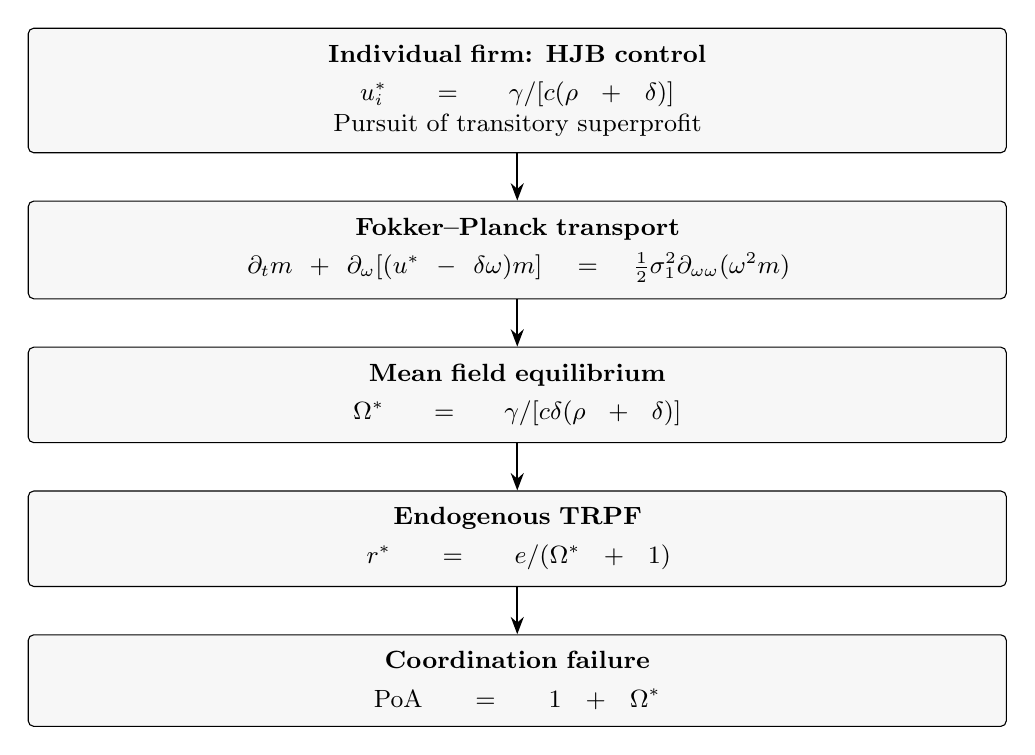
\begin{tikzpicture}[node distance=6mm]
\node[flowbox] (n0) {\textbf{Individual firm: HJB control}\\[3pt]$u_i^*=\gamma/[c(\rho+\delta)]$\\Pursuit of transitory superprofit};
\node[flowbox,below=of n0] (n1) {\textbf{Fokker--Planck transport}\\[3pt]$\partial_t m+\partial_\omega[(u^*-\delta\omega)m]=\frac12\sigma_1^2\partial_{\omega\omega}(\omega^2m)$};
\draw[flowarrow] (n0) -- (n1);
\node[flowbox,below=of n1] (n2) {\textbf{Mean field equilibrium}\\[3pt]$\Omega^*=\gamma/[c\delta(\rho+\delta)]$};
\draw[flowarrow] (n1) -- (n2);
\node[flowbox,below=of n2] (n3) {\textbf{Endogenous TRPF}\\[3pt]$r^*=e/(\Omega^*+1)$};
\draw[flowarrow] (n2) -- (n3);
\node[flowbox,below=of n3] (n4) {\textbf{Coordination failure}\\[3pt]$\mathrm{PoA}=1+\Omega^*$};
\draw[flowarrow] (n3) -- (n4);
\end{tikzpicture}
\caption{The micro-to-macro accumulation mechanism.}
\end{figure}
\subsection{The Bridge to Article 2: From Real Over-Accumulation to Fictitious Capital}
Article 1 established the micro-to-macro trajectory of the real circuit of capital ($M \to C \dots P \dots C' \to M'$). However, the systemic consequences of the TRPF do not remain confined to production:

\begin{enumerate}
\item \textbf{The Profit-Squeeze on Debt Service:} As the real rate of profit ${r}^{*}$ decays, industrial capitals cannot cover fixed contractual debt service out of retained surplus-value (${\Sigma }_{t}$).
\item \textbf{The Fictitious Escape Hatch ($D-D'$):} Faced with falling real returns in production, money-capital detaches from the real circuit and flows into speculative financial paper, credit expansion, and synthetic derivatives.
\item \textbf{The Credit Default Surface:} The upward-drifting organic composition ${\Omega }_{t}$ and the expanding Cost of Anarchy ($PoA$) dynamically push the debt default barrier ${H}_{i}(t)$ upward.
\end{enumerate}
\textbf{Article 2} will formalize this financialized layer: constructing the stochastic credit pricing PDE for corporate debt and CDS contracts, proving that under the TRPF, the equivalent martingale measure $Q$ enforces an inevitable structural default horizon.

\chapter{Fictitious Capital, Measure Changes, and Structural Credit Risk under the TRPF}
\section{Introduction: From Industrial Accumulation to Financial Valuation}
In Article 1, we established that decentralized competition for superprofits forces individual firms to over-accumulate constant capital, driving the systemic organic composition toward its saturation limit ${\Omega }^{*}$ and depressing the real baseline rate of profit:

\[
{r}^{*}=\frac{e}{{\Omega }^{*}+1}
\]
Article 2 examines what happens when this productive circuit ($M \to C \dots P \dots C' \to M'$) is coupled to a financial superstructure ($M\rightarrow M'$). In \emph{Capital Vol. III} (Ch. 21--29), Marx terms financial instruments---shares, sovereign debt, corporate bonds, and secondary derivatives---\textbf{fictitious capital} (\emph{fiktives Kapital}). These assets are not real value in themselves; they are legal titles of ownership that represent claims on future flows of surplus-value ($\Sigma$).

In orthodox mathematical finance, the pricing of these claims is governed by the existence of an equivalent martingale measure $Q$, constructed via Girsanov's theorem, which aligns all expected asset drifts with an exogenous risk-free rate ${r}_{f}$.

Our goal here is to deconstruct this financial architecture from a Marxian perspective:

\begin{enumerate}
\item \textbf{The Conceptual Duality:} We contrast the \textbf{microeconomic stochastic control problem} of the firm (which internalizes diffusion volatility $\sigma$ through quadratic installation costs and volatility penalties) against the \textbf{macroeconomic change of measure} (which re-weights path space to equate heterogeneous valorization drifts to the baseline financial rate of interest).
\item \textbf{The Transformation from Abstract Surplus to the Rate of Interest:} We demonstrate that the shift from the physical measure $P$ to the risk-neutral measure $Q$ is the continuous-time mathematical equivalent of the Marxian transformation of surplus-value into the general rate of profit and its subsequent bifurcation into \textbf{profit of enterprise} and \textbf{interest}.
\item \textbf{The Material Default Boundary:} By anchoring financial asset payouts to actual surplus extraction, we derive a credit pricing PDE where default is governed not by an arbitrary equity threshold, but by the material breakdown of valorization when debt service outstrips extracted surplus-value.
\end{enumerate}
\section{Microeconomic Volatility Adjustment vs. Macroeconomic Measure Change}
A core conceptual divergence between neoclassical economics and financial mathematics lies in how uncertainty is treated at the micro versus macro levels:

\begingroup\small\begin{longtable}{|>{\raggedright\arraybackslash}p{0.20\textwidth}|>{\raggedright\arraybackslash}p{0.34\textwidth}|>{\raggedright\arraybackslash}p{0.34\textwidth}|}\hline
Dimension & Microeconomic Firm Layer (Stochastic Control) & Macroeconomic Valuation Layer (Girsanov Measure Change) \\ \hline
\textbf{Operational Sphere} & Circuit of Productive Capital ($P$) & Circuit of Money/Interest-Bearing Capital ($M-M'$) \\ \hline
\textbf{Mathematical Mechanism} & Dynamic Programming / HJB equation under $P$ & Girsanov transformation from $P\rightarrow Q$ \\ \hline
\textbf{Treatment of Volatility ($\sigma$)} & \textbf{Physical Risk Penalty:} Volatility directly affects variance, capital depletion, and adjustment costs & \textbf{Drift Erasure:} Volatility enters the Girsanov kernel $\theta =\frac{\mu -r}{\sigma }$ to rescale the Radon-Nikodym derivative \\ \hline
\textbf{Objective} & Real surplus-value extraction and superprofit rent capture & Risk-neutral arbitrage-free pricing of paper claims \\ \hline
\end{longtable}\endgroup
\subsection{The Firm's Internalization of Volatility under $P$}
In Article 1, the individual enterprise solves an optimal control problem under the physical measure $P$. Let the firm's capital composition follow:

\[
d{\omega }_{i}(t)=\left({{u}_{i}(t)-\delta {\omega }_{i}(t)}\right)dt+{\sigma }_{1}{\omega }_{i}(t)d{W}_{i,t}^{P}
\]
When the capitalist faces stochastic shocks ${\sigma }_{1}$, the volatility directly affects the firm's cash flows in three concrete ways:

\begin{enumerate}
\item \textbf{Physical Obsolescence Risk:} Random technology shocks expose the firm to down-turns where installed capital becomes obsolete before its value is transferred to the product (\emph{moral depreciation}).
\item \textbf{Jensen's Convexity Effect:} In the HJB equation, the second-order diffusion term $\frac{1}{2}{\sigma }_{1}^{2}{\omega }_{i}^{2}\frac{{\partial }^{2}V}{\partial {\omega }_{i}^{2}}$ shapes the curvature of the value function. If the firm exhibits risk aversion or faces convex financing costs, the capitalist adjusts the control ${u}_{i}^{*}$ directly in response to ${\sigma }_{1}$.
\item \textbf{Operational Precautionary Sizing:} The firm must maintain cash reserves and liquid working capital to prevent liquidity crunches caused by idiosyncratic diffusion shocks $d{W}_{i,t}^{P}$.
\end{enumerate}
At the micro level, \textbf{volatility is an unavoidable physical and operational friction} that cannot be hedged away by diversification; it is borne directly by the industrial enterprise in production.

\subsection{The Macroeconomic Measure Change: Volatility as a Girsanov Normalizer}
In contrast to the production process, financial markets operate at the level of circulating paper titles. Here, the financial system performs an ideological and mathematical abstraction via the Radon-Nikodym derivative:

\[\fitmath{Z_t = \left. \frac{d\mathbb{Q}}{d\mathbb{P}} \right\vert{}_{\mathcal{F}_t} = \exp\left( - \int_0^t \theta_s dW_s^\mathbb{P} - \frac{1}{2} \int_0^t \Vert{}\theta_s\Vert{}^2 ds \right)}\]
where ${\theta }_{t}=\frac{{\mu }_{t}-{r}_{t}}{{\sigma }_{t}}$ is the market price of risk.

Under the Girsanov transformation:

\[
d{W}_{t}^{Q}=d{W}_{t}^{P}+{\theta }_{t}dt
\]
Notice the transformation of role:

\begin{itemize}
\item In production under $P$, $\sigma$ represents real friction and destructive turbulence.
\item In finance under $Q$, $\sigma$ serves purely as a \textbf{normalizing denominator} that scales the drift adjustment ${\theta }_{t}dt$.
\item The transformation $P\rightarrow Q$ algebraically erases the real, idiosyncratic profit drift ${\mu }_{i}$ of individual industrial branches, replacing it with a uniform financial benchmark yield ${r}_{t}$.
\end{itemize}
The Girsanov change of measure is therefore the formal mathematical tool through which \textbf{financial capital abstracts away from the concrete material conditions of production}, treating all assets as if they drift at the uniform rate of interest-bearing capital.

\section{The Conceptual Role of the Girsanov Measure Change: The Double Transformation}
In classical Marxism, the transformation of value into market price occurs in two historical and structural steps:

\begin{enumerate}
\item \textbf{First Transformation (Volume III, Part II):} From individual values (labor-times) to \textbf{prices of production}, equalizing heterogeneous profit rates into the \textbf{general rate of profit} $\bar{r}$.
\item \textbf{Second Transformation (Volume III, Part V):} The splitting of surplus-value and the general profit rate into \textbf{profit of enterprise} (retained by the functioning capitalist) and the \textbf{rate of interest} (${r}_{f}$ or $i$, appropriated by money-capital).
\end{enumerate}
The Girsanov change of measure encapsulates both transformations in continuous time.

\begin{figure}[H]\centering
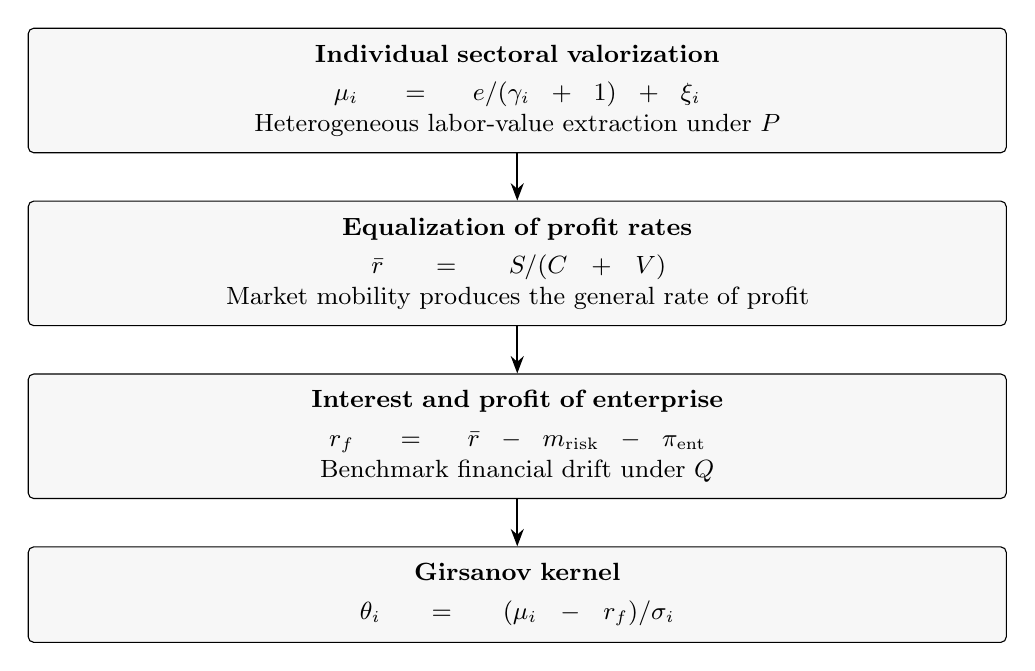
\begin{tikzpicture}[node distance=6mm]
\node[flowbox] (n0) {\textbf{Individual sectoral valorization}\\[3pt]$\mu_i=e/(\gamma_i+1)+\xi_i$\\Heterogeneous labor-value extraction under $P$};
\node[flowbox,below=of n0] (n1) {\textbf{Equalization of profit rates}\\[3pt]$\bar r=S/(C+V)$\\Market mobility produces the general rate of profit};
\draw[flowarrow] (n0) -- (n1);
\node[flowbox,below=of n1] (n2) {\textbf{Interest and profit of enterprise}\\[3pt]$r_f=\bar r-m_{\mathrm{risk}}-\pi_{\mathrm{ent}}$\\Benchmark financial drift under $Q$};
\draw[flowarrow] (n1) -- (n2);
\node[flowbox,below=of n2] (n3) {\textbf{Girsanov kernel}\\[3pt]$\theta_i=(\mu_i-r_f)/\sigma_i$};
\draw[flowarrow] (n2) -- (n3);
\end{tikzpicture}
\caption{The two transformations and their measure-change representation.}
\end{figure}
\subsection{The First Stage: Equalization of Heterogeneous Profit Drifts}
Let the economy comprise $n$ branches of production. Under the physical measure $P$, branch $i$ has organic composition ${\gamma }_{i}={c}_{i}/{v}_{i}$. The real expected profit drift is:

\[
{\mu }_{i}(t)=\frac{{e}_{t}}{{\gamma }_{i,t}+1}+{\xi }_{i,t}
\]
Because ${\gamma }_{i}\ne {\gamma }_{j}$, the physical measure exhibits severe drift heterogeneity.

In Marxian theory, capital mobility between sectors enforces the formation of the general rate of profit:

\[
{\bar{r}}_{t}=\frac{\sum_{i}{S}_{i}(t)}{\sum_{i}({C}_{i}(t)+{V}_{i}(t))}
\]
Capital flowing out of low-profit (high-composition) sectors into high-profit (low-composition) sectors modifies market prices relative to values.

In continuous-time asset pricing, this equalization is executed by projecting asset dynamics onto an equivalent measure where branch-specific valorization advantages are removed.

\subsection{The Second Stage: The Partition into Interest and Profit of Enterprise}
Surplus-value does not remain undivided in the hands of the industrial firm. In \emph{Capital Vol. III}, Ch. 21, Marx demonstrates that gross profit $\bar{r}$ divides qualitatively into:

\[
\bar{r}=i+{p}_{e}
\]
where:

\begin{itemize}
\item $i$: The \textbf{rate of interest}, the baseline return paid to the mere ownership of capital as property (\emph{Kapital als Eigentum}).
\item ${p}_{e}$: The \textbf{profit of enterprise}, the residual return accruing to the functioning industrial capitalist (\emph{fungierender Kapitalist}) as the organizer of the exploitation process.
\end{itemize}
In mathematical finance, the numéraire asset is the money-market account:

\[
d{B}_{t}={r}_{t}{B}_{t}dt
\]
where ${r}_{t}$ is the risk-free rate of interest.

The Girsanov kernel $\theta_t = (\theta_{1,t}, \dots, \theta_{n,t})^\top$ reflects both transformations:

\[\fitmath{\theta_{i,t} = \frac{1}{\sigma_{i,t}} \left[ \underbrace{\left(\frac{e_t}{\gamma_{i,t} + 1} - \bar{r}_t\right)}_{\text{Branch surplus redistribution}} + \underbrace{(\bar{r}_t - r_t)}_{\text{Profit of Enterprise } (p_e)} + \xi_{i,t} \right]}\]
\subsubsection{The Ideological Inversion of the $Q$-Measure}
Under the risk-neutral measure $Q$, every asset drifts at the rate of interest:

\[
\mathbb{E}^\mathbb{Q}\left[ \left. \frac{dS_{i,t}}{S_{i,t}} \right\vert{} \mathcal{F}_t \right] = r_t dt
\]
This produces the core illusion of \textbf{capital fetishism} ($M-M'$):

\begin{enumerate}
\item \textbf{Naturalization of Interest:} Under $Q$, money appears to generate interest autonomously, independent of production.
\item \textbf{Concealment of Living Labor:} The labor-time parameters (${l}_{i}$), the rate of exploitation ($e$), and the organic compositions (${\gamma }_{i}$) disappear from the pricing equations, subsumed entirely into the discount factor ${e}^{-\int{r}_{s}ds}$.
\item \textbf{The Girsanov Shift as Surplus Transfer:} The Radon-Nikodym derivative $\frac{dQ}{dP}$ is the formal probabilistic operator that converts the real world of \emph{surplus-value production} into the secondary realm of \emph{pure financial claim circulation}.
\end{enumerate}
\section{The Structural Crisis of the Measure Change under the TRPF}
In neoclassical mathematical finance, the existence of an equivalent martingale measure $Q$ is guaranteed as long as the market satisfies the No Free Lunch with Vanishing Risk (NFLVR) condition (Delbaen \& Schachermayer, 1994).

However, Novikov's condition requires that the Girsanov kernel be square-integrable:

\[
{E}^{P}\left[{\exp \left({\frac{1}{2}\int\limits_{0}^{T}\parallel {\theta }_{t}\parallel {}^{2}dt}\right)}\right]<\infty
\]
We now examine how the macroeconomic dynamics of Article 1 undermine this condition.

\subsection{Divergence of the Market Price of Risk Kernel}
From Article 1, competitive automation drives the systemic organic composition toward saturation:

\[
\lim\limits_{{t} \rightarrow {\infty }}{\Omega }_{t}={\Omega }^{*}=\frac{\gamma }{c\delta (\rho +\delta )}
\]
which compresses the real systemic rate of profit:

\[
\lim\limits_{{t} \rightarrow {\infty }}{\bar{r}}_{t}={r}^{*}=\frac{e}{{\Omega }^{*}+1}
\]
Now consider the financial sector. Financial liabilities (corporate debt, bank credit, pension claims) are issued with contractual coupon yields ${r}_{\mathrm{debt}}$ that compound exponentially. If the financial rate of interest demands a minimum positive return ${r}_{target}>0$ to prevent debt deflation and liquidation:

\[
{r}_{t}\geq {r}_{\min}>0
\]
As the TRPF takes hold and the real valorization rate falls below the financial interest rate:

\[
\bar{r}_t < r_t \implies p_{e,t} = \bar{r}_t - r_t < 0
\]
The profit of enterprise turns negative: \textbf{the real surplus extracted in production is insufficient to cover the contractual interest claims of finance capital}.

Examine the Girsanov kernel for an industrial capital:

\[
{\theta }_{i,t}=\frac{{\mu }_{i,t}-{r}_{t}}{{\sigma }_{i,t}}=\frac{1}{{\sigma }_{i,t}}\left({\frac{{e}_{t}}{{\gamma }_{i,t}+1}-{r}_{t}}\right)
\]
As mechanization proceeds (${\gamma }_{i}\rightarrow \infty$) or exploitation hits its physical ceiling (${e}_{t}\leq {e}_{\max}$):

\[
{\mu }_{i,t}\rightarrow 0
\]
While finance capital demands ${r}_{t}\geq {r}_{\min}>0$. Consequently:

\[
\parallel {\theta }_{i,t}\parallel \rightarrow \frac{{r}_{\min}}{{\sigma }_{i,t}}>0\quad\text{with constant sign}
\]
If debt compounding forces debt service to escalate while surplus-value generation halts (${\Sigma }_{t}\rightarrow 0$), the financial wedge required to artificially maintain asset prices at their paper valuations diverges:

\[
\parallel {\theta }_{t}\parallel \rightarrow \infty
\]
When $\parallel {\theta }_{t}\parallel \rightarrow \infty$:

\[\fitmath{\int_0^T \Vert{}\theta_t\Vert{}^2 dt \to \infty \implies \mathbb{E}^\mathbb{P}\left[ \exp\left(\frac{1}{2}\int_0^T \Vert{}\theta_t\Vert{}^2 dt\right) \right] = \infty}\]
The equivalent martingale measure $Q$ ceases to be equivalent to $P$ ($\mathbb{Q} \not\ll \mathbb{P}$). The financial system can no longer price claims as martingales: \textbf{the fictitious capital structure collapses into an endogenous realization and credit crisis}.

\section{The Micro Credit Pricing PDE under the Material Default Boundary}
We now derive the contingent claim pricing PDE for a defaultable corporate liability issued by enterprise $i$, embedding the macro-micro coupling developed across Articles 1 and 2.

\subsection{State Variables and Dynamics under $Q$}
The firm's financial viability depends on two coupled state variables:

\begin{enumerate}
\item \textbf{Micro Technological State:} The firm's private organic composition ${\omega }_{i}(t)$.
\item \textbf{Macro Valorization State:} The systemic average rate of profit ${\bar{r}}_{t}$, governed by the TRPF from Article 1.
\end{enumerate}
Under the risk-neutral measure $Q$, by Girsanov's theorem:

\[\fitmath{d{\omega }_{i}(t)=\left[{\frac{\gamma }{c(\rho +\delta )}-(\delta +\gamma ){\omega }_{i}(t)+\gamma {\Omega }_{t}}\right]dt+{\sigma }_{1}{\omega }_{i}(t)d{W}_{i,t}^{Q}}\]
\[
d{\bar{r}}_{t}=-{\kappa }_{r}({\bar{r}}_{t}-{r}^{*})dt+{\sigma }_{r}{\bar{r}}_{t}d{W}_{r,t}^{Q}
\]
with cross-variation $d\langle W_i^\mathbb{Q}, W_r^\mathbb{Q} \rangle_t = \rho_{ir} dt$.

\subsection{The Material Default Stopping Time}
In standard Merton (1974) structural credit risk models, default occurs when equity asset value drops below debt principal: ${V}_{t}\leq D$. But equity market capitalizations are themselves fictitious prices determined within the financial sphere.

In our Marxian framework, default is grounded in the \textbf{material reproduction of industrial capital}:

\begin{itemize}
\item Instantaneous gross surplus-value extracted by firm $i$:
\[
{\Sigma }_{i}(t)=\left[{{\bar{r}}_{t}+\gamma ({\omega }_{i}(t)-{\Omega }_{t})}\right]({\omega }_{i}(t)+1){V}_{i}
\]
\item Mandatory defensive capital expenditure (from Article 1, Section 4):
\[
{I}_{i}^{*}=\frac{1}{2}c({u}_{i}^{*}{)}^{2}=\frac{{\gamma }^{2}}{2c(\rho +\delta {)}^{2}}
\]
\item Contractual debt service due to finance capital:
\[
{\delta }_{i}(t)=({c}_{\mathrm{coupon}}+{\alpha }_{amort}){D}_{i}
\]
\end{itemize}
Free surplus-value available for debt service is:

\[
FS{V}_{i}(t)={\Sigma }_{i}(t)-{I}_{i}^{*}
\]
Default occurs at the first hitting time ${\tau }_{i}$ when extracted surplus fails to cover contractual debt payments:

\[
{\tau }_{i}=\inf \left\{{t\geq 0:FS{V}_{i}(t)\leq {\delta }_{i}(t)}\right\}
\]
This defines a state-dependent \textbf{critical technological default barrier} ${H}_{i}({\bar{r}}_{t},{\Omega }_{t})$:

\[\fitmath{{H}_{i}({\bar{r}}_{t},{\Omega }_{t})={\Omega }_{t}-\frac{1}{\gamma }\left[{{\bar{r}}_{t}-\frac{{\delta }_{i}(t)+\frac{{\gamma }^{2}}{2c(\rho +\delta {)}^{2}}}{({\Omega }_{t}+1){V}_{i}}}\right]}\]
Default occurs whenever the firm's composition falls below this frontier:

\[
{\tau }_{i}=\inf \left\{{t\geq 0:{\omega }_{i}(t)\leq {H}_{i}({\bar{r}}_{t},{\Omega }_{t})}\right\}
\]
\subsection{Derivation of the Credit Pricing PDE}
Let ${M}_{i}({\omega }_{i},\bar{r},t)$ be the arbitrage-free market value of a credit claim (e.g., corporate bond or credit default swap protection leg) issued by firm $i$.

Under $Q$, discounting at the systemic interest rate ${r}_{t}=\bar{r}$ (or a baseline benchmark ${r}_{f}$), the discounted gain process must be a martingale:

\[\fitmath{{E}^{Q}\left[{d\left({{e}^{-\int\limits_{0}^{t}{\bar{r}}_{s}ds}{M}_{i}({\omega }_{i},\bar{r},t)}\right)}\right]+{e}^{-\int\limits_{0}^{t}{\bar{r}}_{s}ds}{\phi }_{i}({\omega }_{i},\bar{r},t)dt=0}\]
where ${\phi }_{i}$ is the continuous cash flow payout rate (coupons).

Applying Itô's Lemma to ${M}_{i}({\omega }_{i},\bar{r},t)$:

\[\fitmath{\begin{aligned} \frac{\partial M_i}{\partial t} &+ \frac{1}{2} \sigma_1^2 \omega_i^2 \frac{\partial^2 M_i}{\partial \omega_i^2} + \rho_{ir} \sigma_1 \sigma_r \omega_i \bar{r} \frac{\partial^2 M_i}{\partial \omega_i \partial \bar{r}} + \frac{1}{2} \sigma_r^2 \bar{r}^2 \frac{\partial^2 M_i}{\partial \bar{r}^2} \\ &+ \left[ \frac{\gamma}{c(\rho + \delta)} - (\delta + \gamma)\omega_i + \gamma \Omega_t \right] \frac{\partial M_i}{\partial \omega_i} - \kappa_r (\bar{r} - r^*) \frac{\partial M_i}{\partial \bar{r}} - \bar{r} M_i + \phi_i(\omega_i, \bar{r}, t) = 0 \end{aligned}}\]
\subsubsection{Boundary Conditions:}
\begin{enumerate}
\item \textbf{At the Valorization Default Barrier (${\omega }_{i}={H}_{i}(\bar{r},\Omega )$):}
\[
{M}_{i}({H}_{i},\bar{r},t)=R(\bar{r})\cdot {D}_{i}
\]
where the recovery rate $R(\bar{r})={R}_{0}{\left({\frac{\bar{r}}{{r}_{0}}}\right)}^{\zeta }$ incorporates the devalorization of fixed constant capital during a systemic profitability crisis.
\item \textbf{At High Innovation States (${\omega }_{i}\rightarrow \infty$):}
The firm commands vast superprofits; default probability vanishes:
\[
{M}_{i}({\omega }_{i},\bar{r},t)\rightarrow {D}_{i}\left[{\frac{{c}_{\mathrm{coupon}}}{\bar{r}}+\left({1-\frac{{c}_{\mathrm{coupon}}}{\bar{r}}}\right){e}^{-\bar{r}(T-t)}}\right]
\]
\item \textbf{Terminal Maturity ($t=T$):}
\[
{M}_{i}({\omega }_{i},\bar{r},T)={D}_{i}\quad\text{for }{\omega }_{i}>{H}_{i}
\]
\end{enumerate}
\section{Synthesis: The Contradiction Between Production and Finance}
Article 2 formalizes the structural tension between real value creation and financial valuation:

\begin{figure}[H]\centering
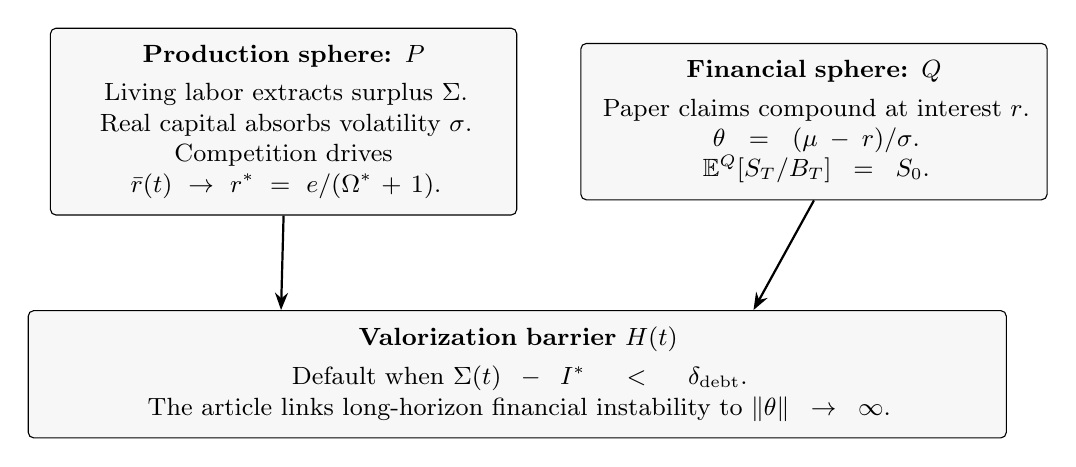
\begin{tikzpicture}[node distance=6mm]

\node[halfbox] (p) {\textbf{Production sphere: $P$}\\[3pt]
Living labor extracts surplus $\Sigma$.\\Real capital absorbs volatility $\sigma$.\\
Competition drives $\bar r(t)\to r^*=e/(\Omega^*+1)$.};
\node[halfbox,right=8mm of p] (q) {\textbf{Financial sphere: $Q$}\\[3pt]
Paper claims compound at interest $r$.\\$\theta=(\mu-r)/\sigma$.\\
$\mathbb E^Q[S_T/B_T]=S_0$.};
\node[flowbox,below=12mm of p.south east,anchor=north] (b) {\textbf{Valorization barrier $H(t)$}\\[3pt]
Default when $\Sigma(t)-I^*<\delta_{\mathrm{debt}}$.\\
The article links long-horizon financial instability to $\lVert\theta\rVert\to\infty$.};
\draw[flowarrow] (p.south) -- ([xshift=-3cm]b.north);
\draw[flowarrow] (q.south) -- ([xshift=3cm]b.north);

\end{tikzpicture}
\caption{Production and finance meet at the material default boundary.}
\end{figure}
\begin{enumerate}
\item \textbf{At the Micro Level:} The individual firm cannot escape diffusion shocks ${\sigma }_{1}$; it internalizes them through real capital expenditures, defensive capex, and operational cushions under $P$.
\item \textbf{At the Macro Level:} The Girsanov change of measure re-weights path space, projecting the illusion that all assets naturally grow at the uniform rate of interest $r$, divorcing financial expectations from living labor.
\item \textbf{The Terminal Breakdown:} Because the TRPF relentlessly compresses real surplus-value ${\bar{r}}_{t}\rightarrow {r}^{*}$, the financial rate of return cannot be sustained out of productive valorization. As the Cost of Anarchy ($PoA$) drives the default boundary ${H}_{i}$ upward, the distance-to-default contracts, credit default spreads diverge, and the mathematical equivalence of the risk-neutral measure $Q$ breaks down.
\end{enumerate}
\chapter{Networked Valorization Crises: Inter-Departmental Credit Contagion and the Topology of Capitalist Devalorization}
\section{The Dual Circuit Network Topology: Physical Input-Output and the Fictitious Credit Layer}
In neoclassical general equilibrium and standard corporate network models, the economic topology is flattened into an exchange web where financial liabilities and goods transactions operate on the same ontological plane. In contrast, Marxian political economy demands a rigorous distinction between two interdependent, structurally asymmetric circuits:

\begin{enumerate}
\item \textbf{The Material Circulation of Capital ($M \to C \dots P \dots C' \to M'$):} The physical and value-theoretic flow of intermediate commodities and living labor across branches of production, governed by technological input-output requirements.
\item \textbf{The Circulation of Interest-Bearing and Fictitious Capital ($M \dots M'$):} The reciprocal web of claims, commercial credit, promissory notes, and banking liabilities that circulate above production.
\end{enumerate}
A systemic crisis arises when the physical reproduction conditions of the material circuit become incompatible with the contractual clearing demands of the fictitious credit network.

\subsection{The Material Production Layer: The Extended Reproduction Schemes}
Let the productive economy be partitioned into $n$ sectors, which can be grouped into Marx's two fundamental macroeconomic departments (\emph{Capital Vol. II}, Ch. 20--21):

\begin{itemize}
\item \textbf{Department I (${D}_{I}$):} Production of the means of production (machinery, raw materials, energy, physical infrastructure).
\item \textbf{Department II (${D}_{II}$):} Production of the means of consumption (wage goods and luxury consumption).
\end{itemize}
Let the physical technology of the economy be characterized by:

\begin{itemize}
\item $A=[{a}_{ij}]\in {R}_{+}^{n\times n}$: The Leontief input-output matrix, where ${a}_{ij}$ is the physical quantity of commodity $i$ required to produce one unit of commodity $j$. We assume $A$ is productive ($\rho (A)<1$).
\item $l = (l_1, \dots, l_n) \in \mathbb{R}_{++}^{1 \times n}$: The vector of direct labor coefficients (labor hours per physical unit of output).
\item $x(t) = (x_1(t), \dots, x_n(t))^\top \in \mathbb{R}_{+}^{n \times 1}$: The gross physical output vector at time $t$.
\end{itemize}
\subsubsection{Labor Values and Monetary Expression}
The vector of socially necessary labor times (values) $\lambda \in {R}_{++}^{1\times n}$ embodied in commodities solves the classic Leontief-Marx equation:

\[
\lambda = \lambda A + l \implies \lambda = l (I - A)^{-1}
\]
Using the Monetary Expression of Labor Time (MELT) ${m}_{t}\in {R}_{++}$, the baseline monetary price of output in value terms is ${p}_{v}(t)={m}_{t}\lambda$.

\subsubsection{Sectoral Capital Accounting in the Material Layer}
For each sector $j \in \{1, \dots, n\}$, total capital advanced per period decomposes into:

\begin{itemize}
\item \textbf{Constant Capital Flow (${C}_{j}$):} The value of intermediate inputs consumed:
\end{itemize}
\[
{C}_{j}(t)={p}_{t}\sum\limits_{i=1}^{n}{a}_{ij}{x}_{j}(t)
\]
\begin{itemize}
\item \textbf{Variable Capital Flow (${V}_{j}$):} The nominal wage bill paid to living labor:
\end{itemize}
\[
{V}_{j}(t)={w}_{t}{l}_{j}{x}_{j}(t)
\]
\begin{itemize}
\item \textbf{Surplus-Value Generated (${S}_{j}$):}
\end{itemize}
\[
{S}_{j}(t)=({m}_{t}-{w}_{t}){l}_{j}{x}_{j}(t)={e}_{t}{V}_{j}(t)
\]
where ${e}_{t}=\frac{{m}_{t}-{w}_{t}}{{w}_{t}}$ is the aggregate rate of exploitation.

The sectoral organic composition of capital is:

\[
{\omega }_{j}(t)=\frac{{C}_{j}(t)}{{V}_{j}(t)}=\frac{{p}_{t}\sum\limits_{i=1}^{n}{a}_{ij}}{{w}_{t}{l}_{j}}
\]
\subsubsection{The Two-Department Reproduction Constraint}
In a classical two-department partition ($n=2$), expanded reproduction requires the structural clearing condition:

\[
{C}_{2}(t)+\Delta {C}_{2}(t)={V}_{1}(t)+{S}_{1}^{consumed}(t)+\Delta {V}_{1}(t)
\]
Department II's demand for constant capital must match Department I's expenditure on consumption goods. Any deviation between physical production in Department I and monetary effective demand in Department II forms the structural origin of \textbf{disproportionality}.

\subsection{The Fictitious Credit Layer: The Inter-Firm Debt Web}
In reality, commodities are rarely exchanged against immediate physical cash ($M$). As Marx details in \emph{Capital Vol. III} (Ch. 25, "Credit and Fictitious Capital"), the circulation of commodities is facilitated by \textbf{commercial credit}---producers sell goods to one another against bills of exchange (\emph{Wechsel}), deferred payment obligations, and inter-firm trade credit:

\begin{quote}
\emph{"The mutual claims of the producers against one another, represented by bills of exchange, serve as the actual currency... this credit expands with the mere expansion of the scale of production."}
\end{quote}

Above trade credit sits the \textbf{banking and financial sector}, which discounts these bills, issues credit lines, and leverages loans against physical capital.

\subsubsection{Formalizing the Inter-Firm Financial Topology}
We define the financial credit network as a weighted, directed graph $G=(V,E)$, where the set of nodes $\mathcal{V} = \{1, \dots, n\}$ represents the industrial sectors (or individual conglomerate capitals), and edges $E$ represent gross bilateral debt obligations.

Let $L(t)=[{L}_{ij}(t)]\in {R}_{+}^{n\times n}$ denote the \textbf{nominal claims matrix}:

\begin{itemize}
\item ${L}_{ij}(t)\geq 0$ represents the nominal payment obligation that sector $i$ owes to sector $j$ maturing at or before time $t+dt$.
\item By construction, ${L}_{ii}(t)=0$ (no self-debt).
\end{itemize}
\subsubsection{Total Inflows and Outflows of Contractual Debt}
\textbf{Total Liabilities (Contractual Debt Outflow):}

The total nominal debt service that sector $i$ must pay to all counterparties in the industrial network is:

\[
{\bar{p}}_{i}(t)=\sum\limits_{j=1}^{n}{L}_{ij}(t)+{\delta }_{bank,i}(t)
\]
where ${\delta }_{bank,i}(t)$ represents non-trade debt obligations owed to external commercial banks and bondholders.

\textbf{Total Claims (Anticipated Inflow):}

The nominal volume of trade claims that sector $i$ expects to receive from its debtor sectors is:

\[
{\bar{c}}_{i}(t)=\sum\limits_{k=1}^{n}{L}_{ki}(t)
\]
\subsubsection{The Relative Liabilities Matrix}
Following the financial network formulation of Eisenberg and Noe (2001), define the row-stochastic relative obligation matrix $\Pi (t)=[{\pi }_{ij}(t)]\in [0,1{]}^{n\times n}$:

\[
\pi_{ij}(t) = \begin{cases} \frac{L_{ij}(t)}{\bar{p}_i(t)}, & \text{if } \bar{p}_i(t) > 0 \\ 0, & \text{if } \bar{p}_i(t) = 0 \end{cases}
\]
${\pi }_{ij}(t)$ specifies the proportion of sector $i$'s total debt service directed to counterparty $j$. Under insolvency, available liquidity is apportioned pro-rata according to these weights.

\subsection{Coupling Production to Finance: The Cash-Flow Balance}
The fundamental contradiction of capitalist reproduction sits at the interface between the physical layer and the credit matrix.

\begin{figure}[H]\centering
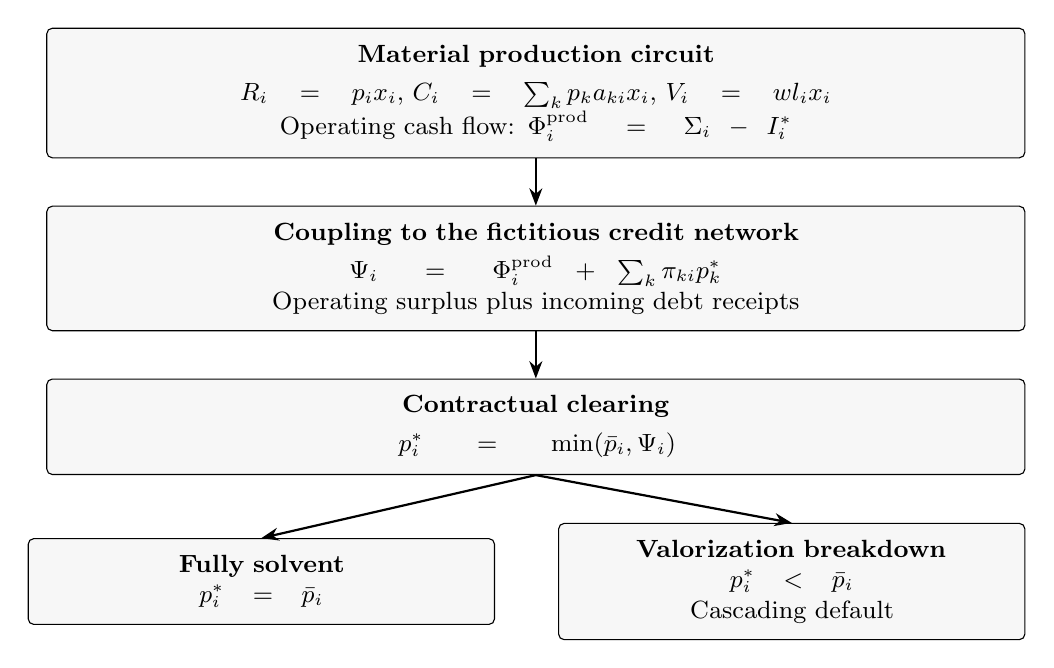
\begin{tikzpicture}[node distance=6mm]

\node[flowbox] (a) {\textbf{Material production circuit}\\[3pt]
$R_i=p_i x_i$, $C_i=\sum_k p_k a_{ki}x_i$, $V_i=w l_i x_i$\\
Operating cash flow: $\Phi_i^{\mathrm{prod}}=\Sigma_i-I_i^*$};
\node[flowbox,below=of a] (b) {\textbf{Coupling to the fictitious credit network}\\[3pt]
$\Psi_i=\Phi_i^{\mathrm{prod}}+\sum_k\pi_{ki}p_k^*$\\Operating surplus plus incoming debt receipts};
\node[flowbox,below=of b] (c) {\textbf{Contractual clearing}\\[3pt]$p_i^*=\min(\bar p_i,\Psi_i)$};
\node[halfbox,below left=8mm and -5.7cm of c] (d) {\textbf{Fully solvent}\\$p_i^*=\bar p_i$};
\node[halfbox,right=8mm of d] (e) {\textbf{Valorization breakdown}\\$p_i^*<\bar p_i$\\Cascading default};
\draw[flowarrow] (a)--(b);\draw[flowarrow] (b)--(c);
\draw[flowarrow] (c.south)--(d.north);\draw[flowarrow] (c.south)--(e.north);

\end{tikzpicture}
\caption{Cash-flow transmission from production to debt clearing.}
\end{figure}
For each sector $i$, the real operating surplus generated in production per unit time (net of the defensive automation expenditure ${I}_{i}^{*}=\frac{{\gamma }_{i}^{2}}{2c(\rho +\delta {)}^{2}}$ derived in Article 1) is:

\[\fitmath{{\Phi }_{i}^{\mathrm{prod}}(t)={\Sigma }_{i}(t)-{I}_{i}^{*}(t)=\left[{{r}_{i}(t)+{\gamma }_{i}({\omega }_{i}(t)-{\Omega }_{t})}\right]({\omega }_{i}(t)+1){V}_{i}(t)-{I}_{i}^{*}(t)}\]
The total liquid cash flow available to sector $i$ to clear its maturing debt obligations ${\bar{p}}_{i}(t)$ is the sum of its \textbf{internally extracted net surplus-value} and its \textbf{actual incoming debt repayments} from other nodes:

\[
{\Psi }_{i}(t)={\Phi }_{i}^{\mathrm{prod}}(t)+\sum\limits_{k=1}^{n}{p}_{k}^{*}(t){\pi }_{ki}(t)
\]
where ${p}_{k}^{*}(t)$ is the actual payment realized by debtor node $k$.

\subsection{Structural Vulnerability of the Dual Network}
The dual circuit exposes the core systemic vulnerability of capitalist financialization:

\textbf{The Nominal Rigidity of the $\Pi$-Matrix:}

Contractual liabilities ${L}_{ij}$ are denominated in nominal money units and fixed by prior legal contracts. They do not automatically contract when physical production stalls.

\textbf{The Stochastic Fragility of the Physical Layer (${\Phi }^{\mathrm{prod}}$):}

Surplus-value extraction ${\Sigma }_{i}(t)$ is subject to:

\begin{itemize}
\item Realization shocks (inability to sell goods at prices of production).
\item Class struggle volatility ($d{e}_{t}$).
\item The secular drag of the TRPF (${\bar{r}}_{t}\rightarrow {r}^{*}$).
\end{itemize}
\textbf{The Leverage Multiplier:}

As long as real surplus-value expands ($\dot{\Sigma }>0$), commercial credit $\Pi$ expands even faster ($M \dots M'$ leverage inflation). But if a valorization shortfall strikes Department I, the real inflow ${\Phi }_{1}^{\mathrm{prod}}$ drops below ${\bar{p}}_{1}$. Because Department I cannot pay its debts to Department II, the shortfall propagates through the matrix $\Pi$, transforming a local crisis of surplus extraction into a generalized network clearing collapse.

\section{Uneven Organic Composition, Sectoral Disproportionality, and the Breakdown of Reproduction}
In Section 1, we defined the dual network coupling physical input-output flows ($A,l$) to inter-firm credit obligations ($\Pi ,L$). We now formalize how the secular increase in the organic composition of capital ($\omega$) does not proceed uniformly across sectors, but develops with severe structural unevenness.

In \emph{Capital Vol. II} (Ch. 20--21) and \emph{Capital Vol. III} (Ch. 15), Marx demonstrates that the reproduction of total social capital requires not merely an aggregate balance of value, but an exact \textbf{material-proportional equivalence} between Department I (Means of Production) and Department II (Means of Consumption). Here, we prove that uneven mechanization endogenously ruptures this proportionality, generating an expanding realization gap that forces the credit network to over-leverage until physical reproduction breaks down.

\subsection{The Asymmetric Composition of Capital: ${\omega }_{1}\gg {\omega }_{2}$}
In industrial capitalism, the technical requirements of production impose an intrinsic asymmetry between the two departments:

\begin{itemize}
\item \textbf{Department I (${D}_{I}$):} Produces heavy machinery, automated fabrication systems, computational infrastructure, and raw materials. To innovate, it must accumulate massive fixed constant capital relative to living labor:
\end{itemize}
\[
{\omega }_{1}(t)=\frac{{C}_{1}(t)}{{V}_{1}(t)}\gg 1
\]
\begin{itemize}
\item \textbf{Department II (${D}_{II}$):} Produces wage goods and consumer commodities. While mechanization occurs, final assembly, customization, services, and perishability keep the living labor requirement per unit of advanced capital structurally higher:
\end{itemize}
\[
{\omega }_{2}(t)=\frac{{C}_{2}(t)}{{V}_{2}(t)}
\]
From Section 4 of Article 1, individual capitals in both departments invest in automation at a rate driven by the superprofit incentive:

\[
{u}_{k}^{*}=\frac{{\gamma }_{k}}{{c}_{k}(\rho +{\delta }_{k})},k\in \{1,2\}
\]
Because Department I produces capital goods directly, its installation friction ${c}_{1}$ is lower and its scale returns to automation ${\gamma }_{1}$ are higher than in Department II (${c}_{1}<{c}_{2}$ and ${\gamma }_{1}>{\gamma }_{2}$). Consequently, the saturation limits and growth rates of the organic composition diverge:

\[
\alpha_{\omega, 1} > \alpha_{\omega, 2} \implies \Omega_1^* \gg \Omega_2^*
\]
This divergence generates an acute divergence in \textbf{direct value profit rates}:

\[
{r}_{1}^{(v)}(t)=\frac{{e}_{t}}{{\omega }_{1}(t)+1}\ll \frac{{e}_{t}}{{\omega }_{2}(t)+1}={r}_{2}^{(v)}(t)
\]
\subsection{The Disproportionality Condition in Expanded Reproduction}
Let total annual gross output in value terms across both departments be:

\[
\begin{aligned} W_1(t) &= C_1(t) + V_1(t) + S_1(t) \\ W_2(t) &= C_2(t) + V_2(t) + S_2(t) \end{aligned}
\]
Under \textbf{expanded reproduction} (\emph{erweiterte Reproduktion}), surplus-value ${S}_{k}$ is partitioned into:

\begin{enumerate}
\item Capitalist unconsumable/reinvested accumulation: ${S}_{k}^{\mathrm{acc}}=\Delta {C}_{k}+\Delta {V}_{k}$.
\item Capitalist unaccumulated luxury consumption: ${S}_{k}^{\mathrm{cons}}=(1-{\kappa }_{k}){S}_{k}$, where ${\kappa }_{k}\in (0,1)$ is the accumulation share.
\end{enumerate}
The material balance of the capitalist economy requires two physical clearing conditions:

\begin{enumerate}
\item \textbf{Department I Output Clearing:} Gross output of means of production must equal total constant capital replacement plus new constant capital accumulation across both departments:
\end{enumerate}
\[
{W}_{1}(t)={C}_{1}(t)+{C}_{2}(t)+\Delta {C}_{1}(t)+\Delta {C}_{2}(t)
\]
\begin{enumerate}
\item \textbf{Department II Output Clearing:} Gross output of consumption goods must equal total wages plus capitalist personal consumption across both departments:
\end{enumerate}
\[
{W}_{2}(t)={V}_{1}(t)+{V}_{2}(t)+{S}_{1}^{\mathrm{cons}}(t)+{S}_{2}^{\mathrm{cons}}(t)+\Delta {V}_{1}(t)+\Delta {V}_{2}(t)
\]
\subsubsection{The Fundamental Reproduction Equality}
Subtracting ${C}_{1}(t)+\Delta {C}_{1}(t)$ from both sides of the Department I clearing equation, we obtain the \textbf{canonical condition for continuous macroeconomic reproduction}:

\[
{C}_{2}(t)+\Delta {C}_{2}(t)={V}_{1}(t)+{S}_{1}^{\mathrm{cons}}(t)+\Delta {V}_{1}(t)
\]
\begin{itemize}
\item \textbf{Left-Hand Side:} Department II's gross demand for new and replacement means of production from Department I.
\item \textbf{Right-Hand Side:} Department I's gross consumer demand for wage goods and consumption commodities from Department II.
\end{itemize}
\subsection{The Realization Gap Induced by the TRPF}
We now evaluate what happens when Department I's organic composition explodes (${\omega }_{1}(t)\rightarrow {\Omega }_{1}^{*}\gg {\Omega }_{2}^{*}$) under the competitive imperatives derived in Article 1.

Let accumulation in each department follow technical proportions:

\[\fitmath{\Delta {C}_{k}(t)={\kappa }_{k}{S}_{k}(t)\left({\frac{{\omega }_{k}(t)}{{\omega }_{k}(t)+1}}\right),\Delta {V}_{k}(t)={\kappa }_{k}{S}_{k}(t)\left({\frac{1}{{\omega }_{k}(t)+1}}\right)}\]
As mechanization accelerates in Department I (${\omega }_{1}(t)\uparrow$):

\textbf{Living Labor Compression in ${D}_{I}$:}

\[
\frac{\Delta {V}_{1}(t)}{{S}_{1}(t)}=\frac{{\kappa }_{1}}{{\omega }_{1}(t)+1}\rightarrow 0
\]
Department I expends an ever-smaller fraction of its surplus-value on variable capital (wages), severely compressing its demand for Department II's consumption goods:

\[
\lim\limits_{{{\omega }_{1}} \rightarrow {\infty }}\left[{{V}_{1}(t)+\Delta {V}_{1}(t)}\right]\ll {C}_{1}(t)
\]
\textbf{Capacity Overhang in ${D}_{I}$:}

Department I's gross physical capacity expands at rate:

\[
\frac{d{W}_{1}}{dt}\propto {C}_{1}(t)+\Delta {C}_{1}(t)\sim O({\omega }_{1})
\]
Department I produces an immense physical volume of machinery and intermediate goods that must be realized through sale.

\textbf{Purchasing Power Deficit in ${D}_{II}$:}

Department II's capacity to absorb Department I's output is bounded by its own available constant capital replacement fund:

\[
{C}_{2}(t)+\Delta {C}_{2}(t)={\omega }_{2}(t){V}_{2}(t)+{\kappa }_{2}{e}_{t}{V}_{2}(t)\left({\frac{{\omega }_{2}}{{\omega }_{2}+1}}\right)
\]
Because Department I purchases fewer and fewer consumer goods from Department II, Department II faces a shortfall in gross money revenue, constraining its ability to purchase Department I's expanded output.

\subsubsection{The Mathematical Realization Gap}
Define the instantaneous realization imbalance $\Xi (t)$:

\[\fitmath{\Xi(t) = \underbrace{\left[ W_1(t) - C_1(t) - \Delta C_1(t) \right]}_{\text{Means of production offered to } \mathcal{D}_{\text{II}}} - \underbrace{\left[ C_2(t) + \Delta C_2(t) \right]}_{\text{Effective purchasing power of } \mathcal{D}_{\text{II}}}}\]
Substituting the accumulation equations:

\[
\Xi (t)=\left({{V}_{1}(t)+{S}_{1}^{\mathrm{cons}}(t)+\Delta {V}_{1}(t)}\right)-\left({{C}_{2}(t)+\Delta {C}_{2}(t)}\right)
\]
Applying Itô's Lemma to the trajectory of $\Xi (t)$ under the stochastic automation paths derived in Article 1:

\[
d\Xi (t)={\mu }_{\Xi }({\omega }_{1},{\omega }_{2})dt+{\sigma }_{\Xi }d{W}_{\Xi ,t}
\]
where the drift satisfies:

\[\fitmath{{\mu }_{\Xi }=\frac{\partial \Xi }{\partial {\omega }_{1}}{\dot{\omega }}_{1}+\frac{\partial \Xi }{\partial {\omega }_{2}}{\dot{\omega }}_{2}<0\quad\text{for }{\omega }_{1}\gg {\omega }_{2}}\]
Because ${\mu }_{\Xi }<0$, a secular \textbf{structural realization deficit} opens:

\[
\mathbb{E}[\Xi(t)] < 0 \implies \text{Overproduction of Means of Production in } \mathcal{D}_{\text{I}}
\]
Department I has produced more machinery than Department II can profitably buy and deploy at reigning prices of production.

\subsection{Fictitious Bridging: The Endogenous Over-Expansion of Inter-Firm Credit}
How does the capitalist system continue to operate when physical reproduction is structurally disproportional ($\Xi (t)<0$)?

It bridges the gap through the \textbf{Fictitious Credit Layer} ($\Pi ,L$) developed in Section 1.

\begin{figure}[H]\centering
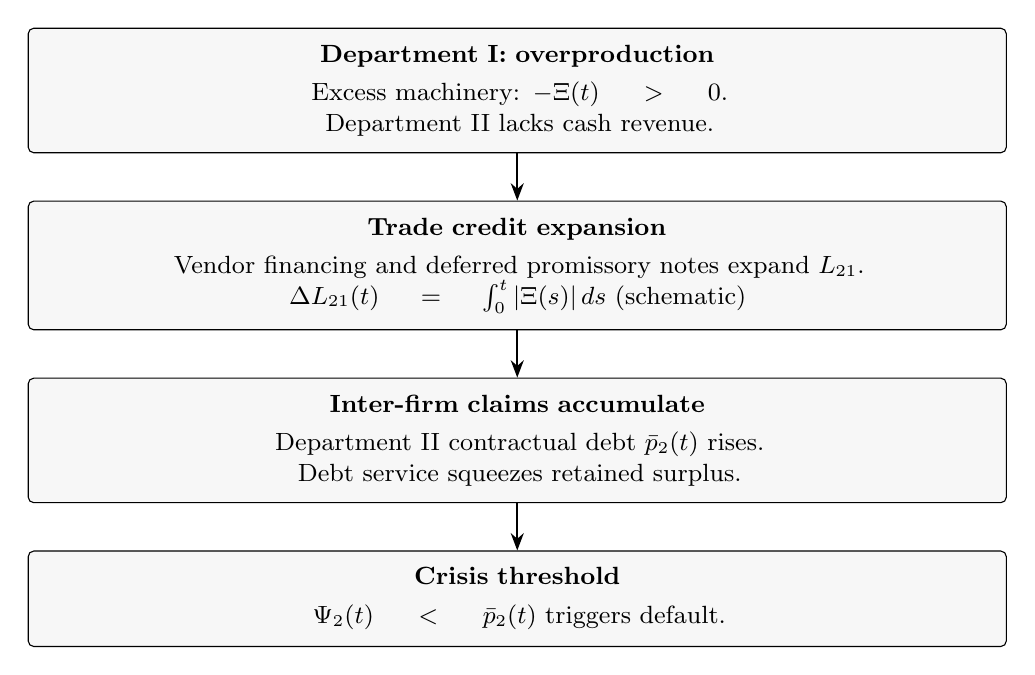
\begin{tikzpicture}[node distance=6mm]
\node[flowbox] (n0) {\textbf{Department I: overproduction}\\[3pt]Excess machinery: $-\Xi(t)>0$.\\Department II lacks cash revenue.};
\node[flowbox,below=of n0] (n1) {\textbf{Trade credit expansion}\\[3pt]Vendor financing and deferred promissory notes expand $L_{21}$.\\$\Delta L_{21}(t)=\int_0^t|\Xi(s)|\,ds$ (schematic)};
\draw[flowarrow] (n0) -- (n1);
\node[flowbox,below=of n1] (n2) {\textbf{Inter-firm claims accumulate}\\[3pt]Department II contractual debt $\bar p_2(t)$ rises.\\Debt service squeezes retained surplus.};
\draw[flowarrow] (n1) -- (n2);
\node[flowbox,below=of n2] (n3) {\textbf{Crisis threshold}\\[3pt]$\Psi_2(t)<\bar p_2(t)$ triggers default.};
\draw[flowarrow] (n2) -- (n3);
\end{tikzpicture}
\caption{Overproduction is bridged by trade credit until the clearing threshold is reached.}
\end{figure}
\textbf{Vendor Financing and Commercial Credit Expansion:}

Unable to sell its surplus equipment for immediate money-capital ($M$), Department I delivers machinery to Department II on credit, accepting deferred payment obligations, bills of exchange, and long-term notes:

\[
\frac{d{L}_{21}(t)}{dt}=\max\left({0,-\Xi (t)}\right)+{g}_{\mathrm{spec}}{L}_{21}(t)
\]
Department II's nominal liabilities owed to Department I (${L}_{21}$) expand continuously to absorb the unsold physical output of Department I.

\textbf{Artificial Prolongation of the Boom:}

On paper, Department I books these credit deliveries as accounts receivable (fictitious asset accumulation: $M \dots M'$). Department I appears profitable and solvent, even though the surplus-value has not been converted into real money (\emph{salto mortale} of the commodity has failed).

\textbf{Escalation of Contractual Debt Service:}

Department II's total contractual debt obligations to the network expand:

\[
{\bar{p}}_{2}(t)={L}_{21}(t)+\sum_{j\ne 1}{L}_{2j}(t)+{\delta }_{bank,2}(t)
\]
While its real operating surplus ${\Phi }_{2}^{\mathrm{prod}}(t)$ is constrained by living labor extraction:

\[
{\Phi }_{2}^{\mathrm{prod}}(t)={e}_{t}{V}_{2}(t)-{I}_{2}^{*}
\]
\subsection{The Mathematical Limit: The Inevitable Rupture}
The ratio of contractual debt obligations to extracted surplus-value in Department II defines its \textbf{fictitious leverage ratio}:

\[
{\Theta }_{2}(t)=\frac{{\bar{p}}_{2}(t)}{{\Phi }_{2}^{\mathrm{prod}}(t)}
\]
Under continuous accumulation:

\begin{itemize}
\item The numerator ${\bar{p}}_{2}(t)$ grows at the rate of capital goods overproduction plus compound interest:
\end{itemize}
\[
\frac{d{\bar{p}}_{2}}{{\bar{p}}_{2}}\sim O\left({\frac{-\Xi (t)}{{\bar{p}}_{2}}+{r}_{\mathrm{debt}}}\right)>0
\]
\begin{itemize}
\item The denominator ${\Phi }_{2}^{\mathrm{prod}}(t)$ is bounded by the TRPF and the biological/social exploitation ceiling:
\end{itemize}
\[
\lim\limits_{{t} \rightarrow {\infty }}{\Phi }_{2}^{\mathrm{prod}}(t)\leq {e}_{\max}{V}_{2}-{I}_{2}^{*}<\infty
\]
Therefore:

\[
\lim_{t \to \tau} \Theta_2(t) = 1 \implies \bar{p}_2(\tau) = \Phi_2^{\text{prod}}(\tau)
\]
At time $\tau$, the entire surplus-value extracted from living labor in Department II is absorbed by debt service. Any negative stochastic shock $d{W}_{t}$ pushes ${\Theta }_{2}(t)>1$, triggering an immediate cash shortfall:

\[
{\Psi }_{2}(t)<{\bar{p}}_{2}(t)
\]
Department II defaults on its commercial obligations to Department I. The fictitious bridge collapses, transforming the structural disproportionality of the physical layer into a \textbf{network-wide financial clearing panic}.

\section{Coupled Network Clearing Dynamics, Eisenberg-Noe Fixed Points, and Cascading Default Thresholds}
Having shown in Section 2 how uneven mechanization (${\omega }_{1}\gg {\omega }_{2}$) generates an expanding realization gap bridged by nominal credit (${L}_{21}\uparrow$), we now formalize the transmission mechanism of the resulting breakdown.

To model the propagation of defaults across the industrial-financial architecture, we adapt the systemic clearing framework of \textbf{Eisenberg and Noe (2001)} to an economy rooted in Marxian surplus-value generation. Unlike orthodox financial network models where operating cash flows are treated as exogenous random endowments, here each node's internal liquidity is explicitly grounded in the real extraction of surplus-value (${\Sigma }_{i}$) derived from living labor.

\subsection{The Network Liquidity Operator}
Consider an economy of $n$ industrial capitals/sectors embedded in the directed inter-firm debt network $(\Pi ,\bar{p})$ established in Section 1:

\begin{itemize}
\item $\bar{p} = (\bar{p}_1, \dots, \bar{p}_n)^\top \in \mathbb{R}_{+}^{n}$: The vector of gross contractual payment obligations due at time $t$.
\item $\Pi =[{\pi }_{ij}]\in [0,1{]}^{n\times n}$: The row-stochastic relative liabilities matrix, where ${\pi }_{ij}={L}_{ij}/{\bar{p}}_{i}$ is the share of sector $i$'s total obligations owed to sector $j$.
\end{itemize}
Let $p^*(t) = (p_1^*(t), \dots, p_n^*(t))^\top \in [0, \bar{p}_1] \times \dots \times [0, \bar{p}_n]$ denote the \textbf{actual clearing payment vector} executed by the network.

\subsubsection{Grounding the External Cash Flow in Surplus Extraction}
In the standard Eisenberg-Noe model, node $i$ receives an arbitrary exogenous cash endowment ${e}_{i}$. In our framework, node $i$'s non-network cash flow is the \textbf{net operating surplus-value} extracted in production:

\[\fitmath{{\Phi }_{i}^{\mathrm{prod}}(t)={\Sigma }_{i}(t)-{I}_{i}^{*}(t)=\left[{{r}_{i}(t)+{\gamma }_{i}({\omega }_{i}(t)-{\Omega }_{t})}\right]({\omega }_{i}(t)+1){V}_{i}(t)-\frac{{\gamma }_{i}^{2}}{2{c}_{i}(\rho +{\delta }_{i}{)}^{2}}}\]
The total liquid cash assets available to sector $i$ at clearing time $t$ equal its extracted surplus plus the actual payments received from its customer and debtor sectors:

\[
{\Psi }_{i}({p}^{*}(t))={\Phi }_{i}^{\mathrm{prod}}(t)+\sum\limits_{j=1}^{n}{\pi }_{ji}{p}_{j}^{*}(t)
\]
In vector notation, letting $\Phi^{\text{prod}}(t) = (\Phi_1^{\text{prod}}(t), \dots, \Phi_n^{\text{prod}}(t))^\top$:

\[
\Psi ({p}^{*}(t))={\Phi }^{\mathrm{prod}}(t)+{\Pi }^{\top }{p}^{*}(t)
\]
\subsection{The Eisenberg-Noe Clearing Fixed Point}
Under standard limited liability and absolute priority (\emph{pari passu} sharing among creditors):

\begin{enumerate}
\item \textbf{Limited Liability:} No sector pays more than its total available liquid assets: ${p}_{i}^{*}(t)\leq {\Psi }_{i}({p}^{*}(t))$.
\item \textbf{Absolute Priority:} If sector $i$ is solvent (${\Psi }_{i}\geq {\bar{p}}_{i}$), it pays its contractual debt in full: ${p}_{i}^{*}(t)={\bar{p}}_{i}$. If sector $i$ is insolvent (${\Psi }_{i}<{\bar{p}}_{i}$), it defaults and surrenders its entire available cash flow to creditors: ${p}_{i}^{*}(t)={\Psi }_{i}({p}^{*}(t))$.
\end{enumerate}
Combining both rules yields the \textbf{nonlinear clearing lattice mapping} ${\Phi }_{clear}:[0,\bar{p}]\rightarrow [0,\bar{p}]$:

\[
p_i^*(t) = \min\left( \bar{p}_i, \; \Phi_i^{\text{prod}}(t) + \sum_{j=1}^n \pi_{ji} \, p_j^*(t) \right), \quad \forall i \in \{1, \dots, n\}
\]
Or in vector form:

\[
{p}^{*}(t)=\bar{p}\wedge \left({{\Phi }^{\mathrm{prod}}(t)+{\Pi }^{\top }{p}^{*}(t)}\right)
\]
where $\wedge$ denotes the element-wise minimum operator.

\subsubsection{Existence and Uniqueness via Tarski's Fixed-Point Theorem}
Define the clearing operator $T:[0,\bar{p}]\rightarrow [0,\bar{p}]$ by:

\[
T(p)=\bar{p}\wedge \left({{\Phi }^{\mathrm{prod}}(t)+{\Pi }^{\top }p}\right)
\]
\begin{enumerate}
\item \textbf{Monotonicity:} Because all entries of $\Pi$ are non-negative (${\pi }_{ji}\geq 0$), $T(p)$ is an order-preserving monotone operator on the complete lattice $[0,\bar{p}]$ under the standard component-wise partial order ($\leq$):
\end{enumerate}
\[
p^{(a)} \le p^{(b)} \implies T(p^{(a)}) \le T(p^{(b)})
\]
\begin{enumerate}
\item \textbf{Fixed-Point Guarantee:} By \textbf{Tarski's Fixed-Point Theorem}, the set of clearing vectors $S=\{p\in [0,\bar{p}]:T(p)=p\}$ is a non-empty, complete lattice. It possesses a unique \textbf{maximal (greatest) clearing vector} ${p}^{*}$, which represents the economically viable market equilibrium reached by continuous debt settlements.
\item \textbf{Regularity Condition:} If every node with a cash shortfall has a directed payment path to an ultimate sink (e.g., net tax outflow or unencumbered capitalist consumption), the spectral radius of the sub-stochastic matrix $\rho ({\Pi }^{\top })<1$, guaranteeing that the clearing vector ${p}^{*}$ is uniquely determined.
\end{enumerate}
\subsection{Partitioning the Network into Solvency and Default Domains}
At clearing time $t$, the clearing vector ${p}^{*}(t)$ partitions the $n$ sectors into two disjoint sets:

\begin{itemize}
\item \textbf{The Solvent Domain (${S}_{t}$):}
\end{itemize}
\[\fitmath{\mathcal{S}_t = \left\{ i \in \{1, \dots, n\} : p_i^*(t) = \bar{p}_i \right\} = \left\{ i : \Phi_i^{\text{prod}}(t) + \sum_{j=1}^n \pi_{ji} p_j^*(t) \ge \bar{p}_i \right\}}\]
\begin{itemize}
\item \textbf{The Default Domain (${D}_{t}$):}
\end{itemize}
\[\fitmath{\mathcal{D}_t = \left\{ i \in \{1, \dots, n\} : p_i^*(t) < \bar{p}_i \right\} = \left\{ i : \Phi_i^{\text{prod}}(t) + \sum_{j=1}^n \pi_{ji} p_j^*(t) < \bar{p}_i \right\}}\]
For any defaulting sector $k\in {D}_{t}$, define its \textbf{clearing shortfall} (nominal debt write-down):

\[
{\Delta }_{k}(t)={\bar{p}}_{k}-{p}_{k}^{*}(t)>0
\]
For sectors in ${D}_{t}$, the clearing equation simplifies to a coupled linear system:

\[
{p}_{D}^{*}(t)={\Phi }_{D}^{\mathrm{prod}}(t)+{\Pi }_{SD}^{\top }{\bar{p}}_{S}+{\Pi }_{DD}^{\top }{p}_{D}^{*}(t)
\]
Solving for the payment vector of defaulting sectors:

\[
{p}_{D}^{*}(t)={\left({I-{\Pi }_{DD}^{\top }}\right)}^{-1}\left({{\Phi }_{D}^{\mathrm{prod}}(t)+{\Pi }_{SD}^{\top }{\bar{p}}_{S}}\right)
\]
The inverse $(I-{\Pi }_{DD}^{\top }{)}^{-1}=\sum\limits_{m=0}^{\infty }({\Pi }_{DD}^{\top }{)}^{m}$ is the \textbf{Leontief-Eisenberg credit multiplier}, which measures the cascade amplification of shortfalls circulating strictly within defaulting capitals.

\subsection{The Cascade Threshold: Propagation from Department II to Department I}
We now connect this network clearing mechanism to the disproportionality dynamics derived in Section 2.

Recall from Section 2.5 that Department II accumulates an unsustainable debt burden to absorb Department I's overproduced machinery:

\[
{\bar{p}}_{2}(t)\uparrow ,\quad\text{while}\quad{\Phi }_{2}^{\mathrm{prod}}(t)={e}_{t}{V}_{2}-{I}_{2}^{*}\quad\text{is bounded by the TRPF}
\]
\subsubsection{Stage 1: The Initial Valorization Failure (Node 2 Enters ${D}_{t}$)}
Default occurs when Department II's isolated surplus fails to cover contractual debt:

\[
{\Phi }_{2}^{\mathrm{prod}}(t)<{\bar{p}}_{2}(t)-\sum_{j\ne 2}{\pi }_{j2}{\bar{p}}_{j}
\]
Department II defaults, generating an initial shortfall:

\[
{\Delta }_{2}(t)={\bar{p}}_{2}-{p}_{2}^{*}(t)>0
\]
\subsubsection{Stage 2: Contagion Feedback to Department I}
Department I relies on incoming payments from Department II to service its own heavy debt obligations (incurred to build automated plant capacity):

\[
{\bar{p}}_{1}(t)=\sum_{j}{L}_{1j}+{\delta }_{bank,1}
\]
Department I's liquid cash flow is:

\[
{\Psi }_{1}(t)={\Phi }_{1}^{\mathrm{prod}}(t)+{\pi }_{21}{p}_{2}^{*}(t)={\Phi }_{1}^{\mathrm{prod}}(t)+{\pi }_{21}({\bar{p}}_{2}-{\Delta }_{2}(t))
\]
Department I remains solvent if and only if ${\Psi }_{1}(t)\geq {\bar{p}}_{1}$.

Therefore, Department I is tipped into default if Department II's shortfall exceeds the \textbf{contagion buffer} of Department I's real operating surplus:

\[
{\Delta }_{2}(t)>\frac{1}{{\pi }_{21}}\left({{\Phi }_{1}^{\mathrm{prod}}(t)+{\pi }_{21}{\bar{p}}_{2}-{\bar{p}}_{1}}\right)
\]

\begin{figure}[H]\centering
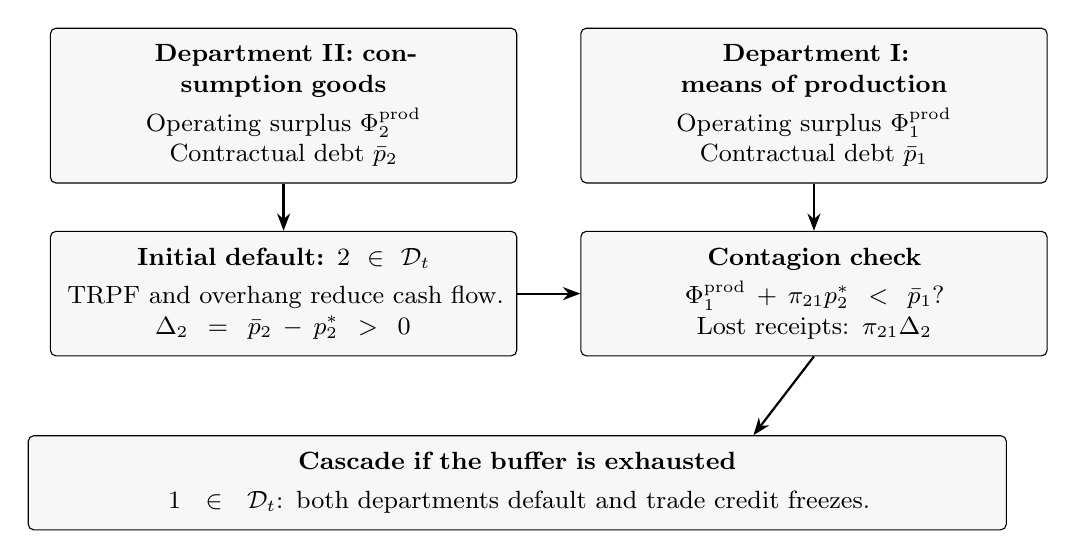
\begin{tikzpicture}[node distance=6mm]

\node[halfbox] (a) {\textbf{Department II: consumption goods}\\[3pt]
Operating surplus $\Phi_2^{\mathrm{prod}}$\\Contractual debt $\bar p_2$};
\node[halfbox,right=8mm of a] (b) {\textbf{Department I: means of production}\\[3pt]
Operating surplus $\Phi_1^{\mathrm{prod}}$\\Contractual debt $\bar p_1$};
\node[halfbox,below=of a] (c) {\textbf{Initial default: $2\in\mathcal D_t$}\\[3pt]
TRPF and overhang reduce cash flow.\\$\Delta_2=\bar p_2-p_2^*>0$};
\node[halfbox,below=of b] (d) {\textbf{Contagion check}\\[3pt]
$\Phi_1^{\mathrm{prod}}+\pi_{21}p_2^*<\bar p_1$?\\Lost receipts: $\pi_{21}\Delta_2$};
\node[flowbox,below=10mm of c.south east,anchor=north] (e) {\textbf{Cascade if the buffer is exhausted}\\[3pt]
$1\in\mathcal D_t$: both departments default and trade credit freezes.};
\draw[flowarrow] (a)--(c);\draw[flowarrow] (b)--(d);
\draw[flowarrow] (c.east)--(d.west);
\draw[flowarrow] (d.south)--([xshift=3cm]e.north);

\end{tikzpicture}
\caption{The reproduction cascade from Department II to Department I.}
\end{figure}
\subsubsection{The Contagion Sensitivity Derivative}
The sensitivity of Department I's clearing payment to an incremental reduction in Department II's surplus extraction (${e}_{2}\downarrow$ or ${w}_{2}\uparrow$) is given by:

\[\fitmath{\frac{\partial p_1^*}{\partial \Phi_2^{\text{prod}}} = \begin{cases} 0, & \text{if } 1 \in \mathcal{S}_t \text{ and } 2 \in \mathcal{S}_t \\ \pi_{21}, & \text{if } 1 \in \mathcal{S}_t \text{ and } 2 \in \mathcal{D}_t \text{ (buffer absorbing shock)} \\ \left[ (I - \Pi_{\mathcal{D}\mathcal{D}}^\top)^{-1} \right]_{12}, & \text{if } \{1, 2\} \subseteq \mathcal{D}_t \text{ (mutual cascade resonance)} \end{cases}}\]
When both departments fall into the default domain ${D}_{t}$, the network multiplier $[(I-{\Pi }_{DD}^{\top }{)}^{-1}{]}_{12}\geq {\pi }_{21}$ amplifies local valorization shortfalls throughout the entire system.

\subsection{Systemic Realization Deficit and Credit Breakdown}
We summarize the core result of Section 3:

\textbf{Theorem 3.1 (Network Valorization Cascade):}

Let the industrial credit network be defined by $(\Pi ,\bar{p})$ with operating cash flows ${\Phi }^{\mathrm{prod}}(t)$ anchored in Marxian surplus extraction.

If the organic composition in Department I drives inter-firm debt beyond the threshold:

\[
{\bar{p}}_{2}(t)>{\Phi }_{2}^{\mathrm{prod}}(t)+\sum_{j\ne 2}{\pi }_{j2}{\bar{p}}_{j}
\]

then Department II defaults. Furthermore, if Department I's real valorization rate satisfies:

\[
{\Phi }_{1}^{\mathrm{prod}}(t)<{\bar{p}}_{1}-{\pi }_{21}{\bar{p}}_{2}+{\pi }_{21}{\Delta }_{2}(t)
\]

then Department I simultaneously defaults.

In this state, the unique Eisenberg-Noe clearing vector ${p}^{*}(t)$ strictly falls below nominal commitments across all sectors (${p}_{i}^{*}(t)<{\bar{p}}_{i},\forall i$), freezing inter-firm trade credit and converting an uneven production crisis into a systemic liquidity panic.

This establishes the formal mechanism: \textbf{financial contagion does not require an exogenous banking shock}---it is the inevitable network consequence of uneven capital composition (${\omega }_{1}\gg {\omega }_{2}$) meeting nominal debt rigidity.

\section{Jump-Diffusions, Endogenous Default Poisson Intensities, and Moral Depreciation (\emph{Entwertung})}
In Section 3, we proved that inter-departmental disproportionality forces the Eisenberg-Noe network clearing vector below contractual commitments (${p}_{i}^{*}(t)<{\bar{p}}_{i}$), freezing trade credit.

However, a capitalist crisis does not stop at an accounting liquidity freeze. In \emph{Capital Vol. III} (Ch. 15, "Internal Contradictions of the Law"), Marx emphasizes that a crisis resolves the contradiction between nominal paper claims and real valorization through \textbf{violent, discrete destruction of value} (\emph{Entwertung} or \emph{moralischer Verschleiß}):

\begin{enumerate}
\item \textbf{Moral Depreciation:} Physical machinery and fixed constant capital are stripped of their book value.
\item \textbf{Bankruptcy Fire-Sales:} Plant, equipment, and inventories are liquidated at distress prices to cover cash obligations.
\item \textbf{Discontinuous Devalorization Jumps:} Value destruction is non-smooth; it arrives as sudden, systemic market seizures.
\end{enumerate}
To capture this mathematically, we transition from pure continuous diffusions to a \textbf{jump-diffusion framework}, where default jump intensities ${\lambda }_{\mathrm{sys}}(t)$ are endogenously driven by the network clearing shortfall derived in Section 3.

\subsection{The Endogenous Crisis Jump Intensity ${\lambda }_{\mathrm{sys}}(t)$}
In neoclassical credit risk modeling (e.g., Duffie-Singleton, Lando), default jump intensities are typically treated as exogenous Cox processes or simple affine functions of arbitrary macroeconomic variables.

In our Marxian framework, default jumps are \textbf{endogenous manifestations of the aggregate clearing deficit}. Define the total systemic payment deficit across the $n$ sectors:

\[
{\Xi }_{\mathrm{def}}(t)=\sum\limits_{i=1}^{n}\max\left({0,{\bar{p}}_{i}(t)-{p}_{i}^{*}(t)}\right)=\sum\limits_{k\in {D}_{t}}^{}{\Delta }_{k}(t)
\]
where ${p}^{*}(t)$ is the maximal Eisenberg-Noe clearing vector and ${D}_{t}$ is the default domain from Section 3.3.

Let $N(t)$ be a point process counting systemic liquidation events, with continuous stochastic intensity ${\lambda }_{\mathrm{sys}}(t)$:

\[
\mathbb{P}\left( N(t + dt) - N(t) = 1 \;\middle\vert\; \mathcal{F}_t \right) = \lambda_{\text{sys}}(t) dt + o(dt)
\]
We formulate ${\lambda }_{\mathrm{sys}}(t)$ as a super-linear function of the relative clearing shortfall:

\[
{\lambda }_{\mathrm{sys}}(t)={\lambda }_{0}\cdot \exp \left({\zeta \cdot \frac{{\Xi }_{\mathrm{def}}(t)}{{\bar{P}}_{\mathrm{total}}(t)}}\right)-{\lambda }_{0}
\]
where:

\begin{itemize}
\item ${\bar{P}}_{\mathrm{total}}(t)=\sum\limits_{i=1}^{n}{\bar{p}}_{i}(t)$ is total nominal debt commitments across the economy.
\item $\zeta >0$ represents the panic elasticity of credit markets (margin calls, collateral seizures).
\item ${\lambda }_{0}>0$ is a baseline hazard scale.
\end{itemize}
\subsubsection{Properties of the Intensity:}
\begin{itemize}
\item \textbf{Fully Solvent State ($\mathcal{D}_t = \emptyset$):} $\Xi_{\text{def}}(t) = 0 \implies \lambda_{\text{sys}}(t) = 0$. In the absence of a clearing shortfall, defaults cannot occur as discontinuous jumps.
\item \textbf{Cascading Breakdown (${\Xi }_{\mathrm{def}}(t)\rightarrow {\bar{P}}_{\mathrm{total}}$):} As the network shortfall approaches total systemic liabilities, ${\lambda }_{\mathrm{sys}}(t)$ diverges exponentially (${\lambda }_{\mathrm{sys}}\rightarrow {\lambda }_{0}({e}^{\zeta }-1)\gg 0$), transforming continuous distress into an immediate, inevitable Poisson arrival.
\end{itemize}
\subsection{Jump Dynamics on Constant Capital: Moral Depreciation}
Let ${C}_{i}(t)={\omega }_{i}(t){V}_{i}(t)$ represent the nominal book value of constant capital (plant, machinery, and equipment) deployed in sector $i$.

Prior to the jump arrival ($dN(t)=0$), ${C}_{i}(t)$ evolves according to the continuous controlled diffusion derived in Article 1:

\[
d{C}_{i}^{c}(t)=\left({{u}_{i}^{*}-\delta {C}_{i}(t)}\right)dt+{\sigma }_{C,i}{C}_{i}(t)d{W}_{i,t}
\]
When a systemic clearing failure triggers a Poisson jump event ($dN(t)=1$), commercial bankruptcy proceedings force immediate liquidation. Sectoral capital goods are dumped onto secondary markets to service creditors, precipitating \textbf{moral depreciation}:

\[
d{C}_{i}(t)=d{C}_{i}^{c}(t)-{J}_{C}(i,{\Xi }_{\mathrm{def}}){C}_{i}({t}^{-})dN(t)
\]
where ${C}_{i}({t}^{-})=\lim\limits_{s\uparrow t}{C}_{i}(s)$ is the pre-jump capital stock, and ${J}_{C}(i,\cdot )\in (0,1)$ is the \textbf{fractional devalorization haircut}.

\subsubsection{The Endogenous Haircut Function}
The magnitude of the price collapse depends directly on the severity of the systemic debt overhang:

\[
{J}_{C}(i,{\Xi }_{\mathrm{def}})=1-\exp \left({-{\theta }_{C}\cdot \frac{{\Xi }_{\mathrm{def}}({t}^{-})}{\sum_{k}{C}_{k}({t}^{-})}}\right),{\theta }_{C}>0
\]
\begin{itemize}
\item If the clearing shortfall is minimal, capital goods retain most of their replacement value (${J}_{C}\approx 0$).
\item If the shortfall is severe, generalized fire-sales cause the market price of specialized machinery to plunge toward scrap metal value:
\[\lim_{\Xi_{\text{def}} \to \infty} J_C = 1 \implies C_i(t) \to 0\]
This directly operationalizes Marx's dictum in \emph{Capital Vol. III}, Ch. 15:
\emph{"A large portion of the nominal capital of the society, i.e., of the exchange-value of the existing capital, is completely destroyed... their value decreases by one third, one half, or more."}
\end{itemize}
\subsection{Jump Dynamics on Fictitious Capital: Debt Cancellation and Repudiation}
The liquidation jump simultaneously strikes the financial credit layer $(\Pi ,L)$. When sector $k\in {D}_{t}$ collapses:

\begin{enumerate}
\item Its outstanding receivables (${L}_{ik}$ for $i\ne k$) become uncollectible bad debts.
\item Its liabilities (${L}_{kj}$) are repudiated or restructured at pennies on the dollar.
\end{enumerate}
Let ${F}_{t}=\sum_{i,j}{L}_{ij}(t)$ denote the total volume of fictitious credit circulating in the inter-firm network. The jump law of motion for total fictitious capital is:

\[
d{F}_{t}=\left({{g}_{F}{F}_{t}}\right)dt-{J}_{F}({\Xi }_{\mathrm{def}}){F}_{{t}^{-}}dN(t)
\]
where the debt cancellation haircut ${J}_{F}\in (0,1]$ satisfies:

\[
{J}_{F}({\Xi }_{\mathrm{def}})=\min\left({1,\frac{{\Xi }_{\mathrm{def}}({t}^{-})}{\sum_{j}{\Phi }_{j}^{\mathrm{prod}}({t}^{-})}}\right)
\]
When the clearing deficit exceeds the aggregate operating surplus of the entire economy (${\Xi }_{\mathrm{def}}>\sum{\Phi }^{\mathrm{prod}}$), the financial superstructure is mathematically insolvent. The jump forces ${J}_{F}\rightarrow 1$: \textbf{generalized debt jubilee through bankruptcy, bank runs, and contractual cancellation}.

\subsection{The Full Master Jump-Diffusion Pricing PDE}
We now incorporate these jump dynamics into the valuation of financial liabilities. Consider a contingent claim $V(C,F,t)$ (e.g., corporate debt or equity in an industrial conglomerate) written on constant capital $C$ and fictitious debt claims $F$.

Under the risk-neutral measure $Q$, the jump intensity is compensated:

\[
d\tilde{N}(t)=dN(t)-{\lambda }_{\mathrm{sys}}^{Q}(t)dt
\]
By Itô's Lemma for semi-martingales with jumps, $V(C,F,t)$ satisfies the \textbf{Partial Integro-Differential Equation (PIDE)}:

\[\fitmath{\begin{aligned} \frac{\partial V}{\partial t} &+ \frac{1}{2} \sigma_C^2 C^2 \frac{\partial^2 V}{\partial C^2} + \rho_{CF} \sigma_C \sigma_F C F \frac{\partial^2 V}{\partial C \partial F} + \frac{1}{2} \sigma_F^2 F^2 \frac{\partial^2 V}{\partial F^2} \\ &+ \mu_C^\mathbb{Q} C \frac{\partial V}{\partial C} + \mu_F^\mathbb{Q} F \frac{\partial V}{\partial F} - \bar{r} V + \phi(C, F, t) \\ &+ \lambda_{\text{sys}}^\mathbb{Q} \cdot \left[ V\left( (1 - J_C)C, \; (1 - J_F)F, \; t \right) - V(C, F, t) \right] = 0 \end{aligned}}\]
\subsubsection{Analysis of the Non-Local Jump Term:}
The term inside the brackets:

\[
{\Delta }_{jump}V=V\left({(1-{J}_{C})C,(1-{J}_{F})F,t}\right)-V(C,F,t)<0
\]
is the \textbf{discrete capital loss} suffered by the financial claim when moral depreciation occurs.

Because ${\lambda }_{\mathrm{sys}}^{Q}\rightarrow \infty$ as the clearing deficit ${\Xi }_{\mathrm{def}}$ mounts, the non-local jump integral dominates standard continuous diffusion hedging:

\begin{itemize}
\item In ordinary times (${\Xi }_{\mathrm{def}}=0$), continuous delta-hedging is possible (${\Delta }_{jump}V\cdot \lambda \approx 0$).
\item In late-stage over-accumulation (${\Xi }_{\mathrm{def}}\gg 0$), risk-neutral market makers cannot hedge the jump risk through continuous trading. \textbf{The pricing PDE breaks down: markets experience liquidity black holes and catastrophic gap risk.}
\end{itemize}
\subsection{The Devalorization Cascade: Summary}

\begin{figure}[H]\centering
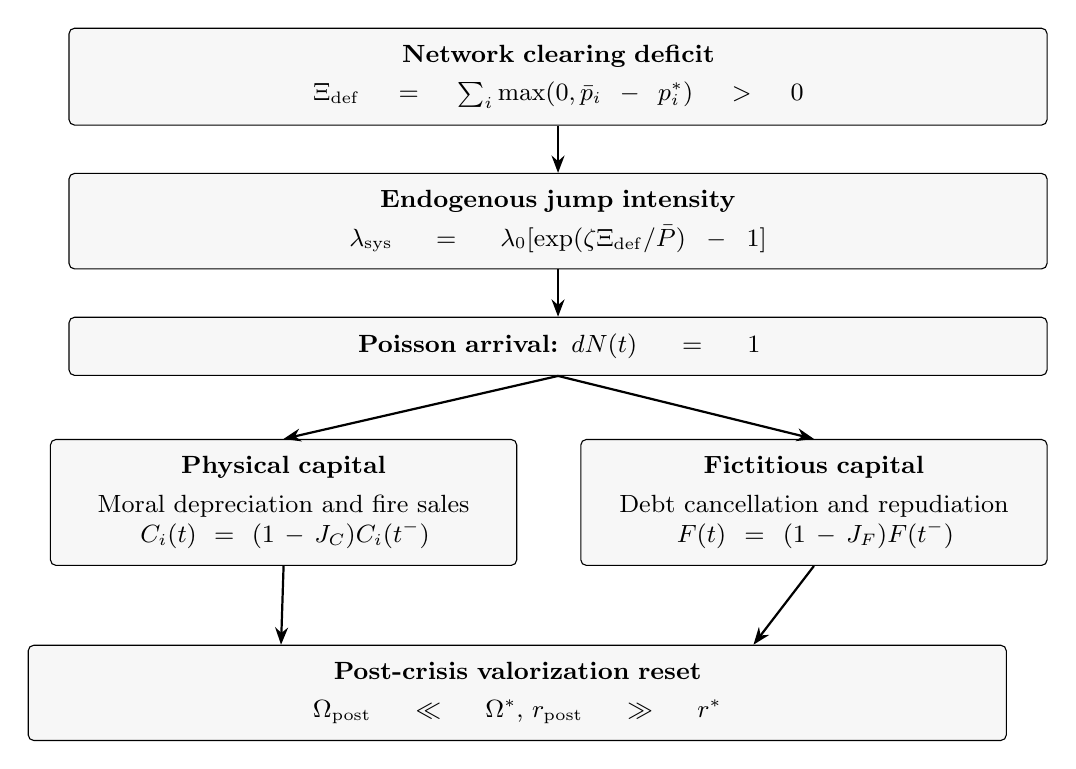
\begin{tikzpicture}[node distance=6mm]

\node[flowbox] (a) {\textbf{Network clearing deficit}\\[3pt]
$\Xi_{\mathrm{def}}=\sum_i\max(0,\bar p_i-p_i^*)>0$};
\node[flowbox,below=of a] (b) {\textbf{Endogenous jump intensity}\\[3pt]
$\lambda_{\mathrm{sys}}=\lambda_0[\exp(\zeta\Xi_{\mathrm{def}}/\bar P)-1]$};
\node[flowbox,below=of b] (c) {\textbf{Poisson arrival: $dN(t)=1$}};
\node[halfbox,below left=8mm and -5.7cm of c] (d) {\textbf{Physical capital}\\[3pt]
Moral depreciation and fire sales\\$C_i(t)=(1-J_C)C_i(t^-)$};
\node[halfbox,right=8mm of d] (e) {\textbf{Fictitious capital}\\[3pt]
Debt cancellation and repudiation\\$F(t)=(1-J_F)F(t^-)$};
\node[flowbox,below=10mm of d.south east,anchor=north] (f) {\textbf{Post-crisis valorization reset}\\[3pt]
$\Omega_{\mathrm{post}}\ll\Omega^*$, $r_{\mathrm{post}}\gg r^*$};
\draw[flowarrow] (a)--(b);\draw[flowarrow] (b)--(c);
\draw[flowarrow] (c.south)--(d.north);\draw[flowarrow] (c.south)--(e.north);
\draw[flowarrow] (d.south)--([xshift=-3cm]f.north);\draw[flowarrow] (e.south)--([xshift=3cm]f.north);

\end{tikzpicture}
\caption{The devalorization cascade and the two capital haircuts.}
\end{figure}
The jump-diffusion framework formalizes Marx's insight: capitalist crises do not follow smooth Gaussian paths. They operate as \textbf{discontinuous topological collapses} where fictitious claims and physical capital are forcibly devalorized to match the underlying surplus-value generated by living labor.

\section{The Post-Crisis Purge, Wage Squeeze, and the Restoration of the Profit Rate}
A capitalist crisis in Marxian political economy is neither an external friction nor a terminal breakdown; it is the \textbf{violent, endogenous mechanism through which capitalist reproduction forcibly restores its own viability}. As Marx summarizes in \emph{Capital Vol. III} (Ch. 15):

\begin{quote}
\emph{"The crisis always forms the starting-point of great new investments. It therefore forms, more or less, the new material basis for the next cycle of turnover."}
\end{quote}

In Section 4, we showed that the arrival of the crisis Poisson jump ($dN(t)=1$) destroys book values via moral depreciation (${J}_{C}$) and cancels nominal claims (${J}_{F}$). We now formalize the subsequent \textbf{post-crisis purge}: the systemic reset of the organic composition of capital ($\Omega$), the expansion of the industrial reserve army of labor, the counter-offensive on the rate of exploitation ($e$), and the mathematical restoration of the general rate of profit ($r$).

\subsection{The Post-Jump Capital Purge: Reset of the Organic Composition}
Prior to the crisis jump at $t=\tau$, the decentralized Mean Field Game (Article 1) had driven the economy-wide average organic composition toward its saturation limit:

\[
\Omega ({\tau }^{-})={\Omega }^{*}=\frac{\gamma }{c\delta (\rho +\delta )}\gg 1
\]
When the systemic default jump occurs ($dN(\tau )=1$), two simultaneous devaluations occur:

\begin{enumerate}
\item \textbf{Physical scrapping and idling:} Less-efficient plant and machinery are abandoned or physically dismantled.
\item \textbf{Moral devaluation:} Bankrupt capital assets are acquired at distress liquidation auctions by surviving capitals at a fraction $(1-{J}_{C})$ of their original value.
\end{enumerate}
Let ${C}_{\mathrm{post}}=(1-{\bar{J}}_{C})C({\tau }^{-})$ denote the post-crisis aggregate constant capital stock, where ${\bar{J}}_{C}\in (0,1)$ is the economy-wide average moral depreciation haircut.

While constant capital suffers immediate discrete destruction, variable capital $V=wL$ cannot contract by an identical proportion if basic physical reproduction continues. Consequently, the \textbf{effective organic composition of capital drops discontinuously}:

\[\fitmath{{\Omega }_{\mathrm{post}}=\frac{{C}_{\mathrm{post}}}{{V}_{\mathrm{post}}}=\frac{(1-{\bar{J}}_{C})C({\tau }^{-})}{V({\tau }^{-})\cdot (1-{\phi }_{L})}={\Omega }^{*}\cdot \left({\frac{1-{\bar{J}}_{C}}{1-{\phi }_{L}}}\right)}\]
where ${\phi }_{L}\in (0,1)$ is the immediate drop in the wage bill due to initial employment contraction.

Because asset write-downs during systemic liquidations vastly outstrip immediate wage-bill reductions (${\bar{J}}_{C}\gg {\phi }_{L}$):

\[
\frac{1 - \bar{J}_C}{1 - \phi_L} < 1 \implies \Omega_{\text{post}} \ll \Omega^*
\]
The devalorization jump mechanically \textbf{cleanses the denominator} of the systemic profit rate.

\subsection{The Industrial Reserve Army and the Wage Squeeze (${e}_{\mathrm{post}}\uparrow$)}
The destruction of constant capital triggers mass bankruptcies, factory closures, and corporate restructurings, unleashing sudden layoffs across both departments.

\subsubsection{Dynamics of the Industrial Reserve Army}
Let ${N}_{\mathrm{total}}$ be the total available labor force, and let $L(t)$ be the actively employed living labor. The \textbf{unemployment rate} (relative size of the industrial reserve army) is:

\[
{u}_{\mathrm{res}}(t)=1-\frac{L(t)}{{N}_{\mathrm{total}}}
\]
At the moment of the crisis jump ($t=\tau$), employment plunges:

\[
L(\tau )=(1-{\chi }_{layoff})L({\tau }^{-}),{\chi }_{layoff}\in (0,1)
\]
causing the reserve army to surge:

\[
{u}_{\mathrm{res}}(\tau )={u}_{\mathrm{res}}({\tau }^{-})+{\chi }_{layoff}(1-{u}_{\mathrm{res}}({\tau }^{-}))\gg {u}_{\mathrm{res}}({\tau }^{-})
\]
\subsubsection{The Marxian Phillips Curve and Wage Repression}
Following the Goodwin (1967) predator-prey formulation, real wage growth is regulated by the disciplinary pressure of the reserve army:

\[
\frac{d{w}_{t}}{{w}_{t}}=\Phi ({u}_{\mathrm{res}}(t))dt+{\sigma }_{w}d{W}_{w,t}
\]
where $\Phi '(\cdot )<0$.

When the reserve army expands abruptly (${u}_{\mathrm{res}}\gg 0$):

\[
\Phi ({u}_{\mathrm{res}}(\tau ))\ll 0
\]
Labor bargaining power collapses. Capital imposes real wage cuts, eliminates benefits, accelerates line speeds, and lengthens unpaid overtime without resistance.

\subsubsection{The Resulting Exploitation Surge}
Recall that the rate of surplus-value is ${e}_{t}=\frac{{m}_{t}-{w}_{t}}{{w}_{t}}=\frac{{m}_{t}}{{w}_{t}}-1$.

As nominal and real wages ${w}_{t}$ are compressed while labor productivity ${m}_{t}$ is enforced through intensified speedups, the rate of exploitation jumps upward:

\[
{e}_{\mathrm{post}}=e(\tau )=\frac{m(\tau )}{w(\tau )}-1\gg e({\tau }^{-})
\]
This formalizes Marx's primary \emph{counteracting influence} (\emph{Capital Vol. III}, Ch. 14): the crisis forcibly raises the rate of surplus-value by depressing wages below the historic value of labor-power.

\subsection{The Mathematical Rebound of the Systemic Rate of Profit}
We can now compute the immediate post-crisis rate of profit ${r}_{\mathrm{post}}$:

\[
{r}_{\mathrm{post}}=\frac{{e}_{\mathrm{post}}}{{\Omega }_{\mathrm{post}}+1}
\]
Comparing ${r}_{\mathrm{post}}$ to the depressed pre-crisis steady state ${r}^{*}=\frac{e({\tau }^{-})}{{\Omega }^{*}+1}$:

\[
\frac{{r}_{\mathrm{post}}}{{r}^{*}}=\left({\frac{{e}_{\mathrm{post}}}{e({\tau }^{-})}}\right)\cdot \left({\frac{{\Omega }^{*}+1}{{\Omega }_{\mathrm{post}}+1}}\right)
\]
Because:

\begin{enumerate}
\item ${e}_{\mathrm{post}}>e({\tau }^{-})$ (Wage repression and labor speedup increase the numerator), and
\item ${\Omega }_{\mathrm{post}}\ll {\Omega }^{*}$ (Moral depreciation and bankruptcies compress the denominator),
\end{enumerate}
both mechanisms act in unison to produce an \textbf{unambiguous, non-linear rebound}:

\[
{r}_{\mathrm{post}}\gg {r}^{*}
\]

\begin{figure}[H]\centering
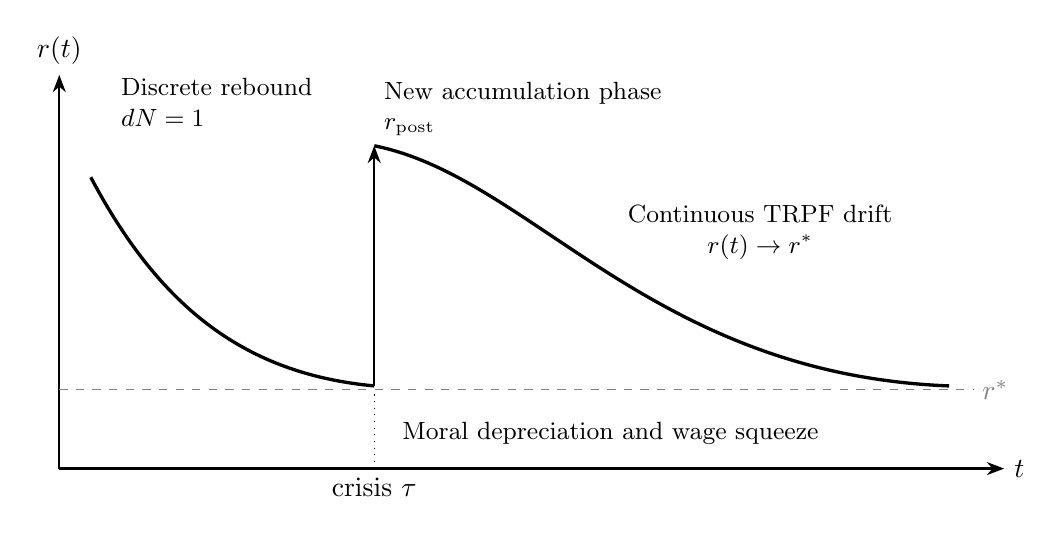
\begin{tikzpicture}[node distance=6mm]

\draw[flowarrow] (0,0)--(12,0) node[right] {$t$};
\draw[flowarrow] (0,0)--(0,5) node[above] {$r(t)$};
\draw[dashed,gray] (0,1)--(11.6,1) node[right] {$r^*$};
\draw[very thick] (0.4,3.7) .. controls (1.3,2) and (2.4,1.2) .. (4,1.05);
\draw[very thick,flowarrow] (4,1.05)--(4,4.1);
\draw[very thick] (4,4.1) .. controls (6,3.7) and (7.5,1.2) .. (11.3,1.05);
\draw[dotted] (4,0)--(4,1);
\node[below] at (4,0) {crisis $\tau$};
\node[above right,align=left,font=\small] at (4,4.1) {New accumulation phase\\$r_{\mathrm{post}}$};
\node[align=center,font=\small] at (8.9,3) {Continuous TRPF drift\\$r(t)\to r^*$};
\node[align=left,font=\small] at (2,4.65) {Discrete rebound\\$dN=1$};
\node[align=center,font=\small] at (7,0.45) {Moral depreciation and wage squeeze};

\end{tikzpicture}
\caption{Schematic profit-rate cycle: continuous decline, crisis jump, and renewed accumulation.}
\end{figure}
\subsection{Deleveraging and the Regeneration of the Credit Network}
The crisis jump similarly purges the fictitious superstructure:

\begin{enumerate}
\item \textbf{Extinction of Insolvent Claims:} Unpayable debts ${L}_{ij}$ are permanently erased via bankruptcies (${J}_{F}\rightarrow 1$).
\item \textbf{Contraction of the Clearing Deficit:}
\end{enumerate}
\[
{\Xi }_{\mathrm{def}}({\tau }^{+})=\sum_{i}\max\left({0,{\bar{p}}_{i}({\tau }^{+})-{p}_{i}^{*}({\tau }^{+})}\right)\rightarrow 0
\]
\textbf{Plunge of the Crisis Hazard Rate:}

Because the clearing deficit collapses to zero, the endogenous jump intensity returns to baseline:

\[
{\lambda }_{\mathrm{sys}}({\tau }^{+})={\lambda }_{0}\left({\exp (0)-1}\right)=0
\]
With nominal debt burdens wiped out and real profit rates restored (${r}_{\mathrm{post}}\gg {r}^{*}$), the distance-to-default ${X}_{t}$ expands dramatically across all surviving firms. Inter-firm trust is re-established, trade credit resumes on a sounder material base, and the equivalent martingale measure $Q$ temporarily regains its operational validity.

\subsection{Limit-Cycle Dynamics: The Endogenous Marxian Metacycle}
The economy has not achieved a static equilibrium; it has merely completed one phase of a continuous, non-linear limit cycle.

Once ${r}_{\mathrm{post}}$ is high and the credit network is purged:

\begin{enumerate}
\item Surplus capital re-enters production.
\item Individual capitals again observe that investing in labor-saving automation yields temporary superprofits:
\end{enumerate}
\[
{u}_{i}^{*}=\frac{\gamma }{c(\rho +\delta )}>0
\]
\begin{enumerate}
\item As atomized firms repeat their HJB-optimal mechanization strategies (Article 1), the Fokker-Planck transport equation begins driving the social composition $\Omega (t)$ upward once more:
\end{enumerate}
\[
\frac{d\Omega }{dt}=\frac{\gamma }{c(\rho +\delta )}-\delta \Omega (t)>0
\]
\begin{enumerate}
\item As $\Omega (t)\rightarrow {\Omega }^{*}$, the systemic profit rate decays, unevenness between departments widens (Section 2), the Eisenberg-Noe clearing vector fails (Section 3), jump hazard ${\lambda }_{\mathrm{sys}}$ spikes (Section 4), and the system plunges toward its next systemic devalorization jump.
\end{enumerate}
The macro-trajectory of capitalist mathematical finance is therefore not a random walk around a stationary Pareto optimum, but an \textbf{endogenous relaxation oscillator} driven by the contradiction between competitive value production and financial claim accumulation.

\section{Full Trilogy Synthesis \& Epistemological Manifesto}
With the derivation of the post-crisis purge and cyclic reset complete, we can synthesize the three articles into a unified mathematical and conceptual architecture.

For nearly half a century, mathematical finance has developed under an axiomatic paradigm borrowed from neoclassical equilibrium theory:

\begin{itemize}
\item Asset prices are driven by exogenous martingales under risk-neutral measures ($Q$).
\item Capital is conceptualized as a physical or monetary stock that continuously bears yield.
\item Volatility is treated as a Gaussian or jump-diffusion perturbation around an efficient market frontier.
\item Crises are modeled as low-probability tail events hitting an otherwise self-correcting system.
\end{itemize}
This trilogy demonstrates that by grounding stochastic calculus, optimal control, and financial network theory in \textbf{Marxian political economy}, mathematical finance can be reconstructed from an apologetic technique of financial engineering into an \textbf{analytical science of systemic contradiction, capital accumulation, and structural crisis}.

\subsection{The Unified Trilogy Architecture}
The three articles form an unbroken progression from the microeconomic behavior of individual industrial firms to macroeconomic credit collapse and systemic regeneration:

\begin{figure}[H]\centering
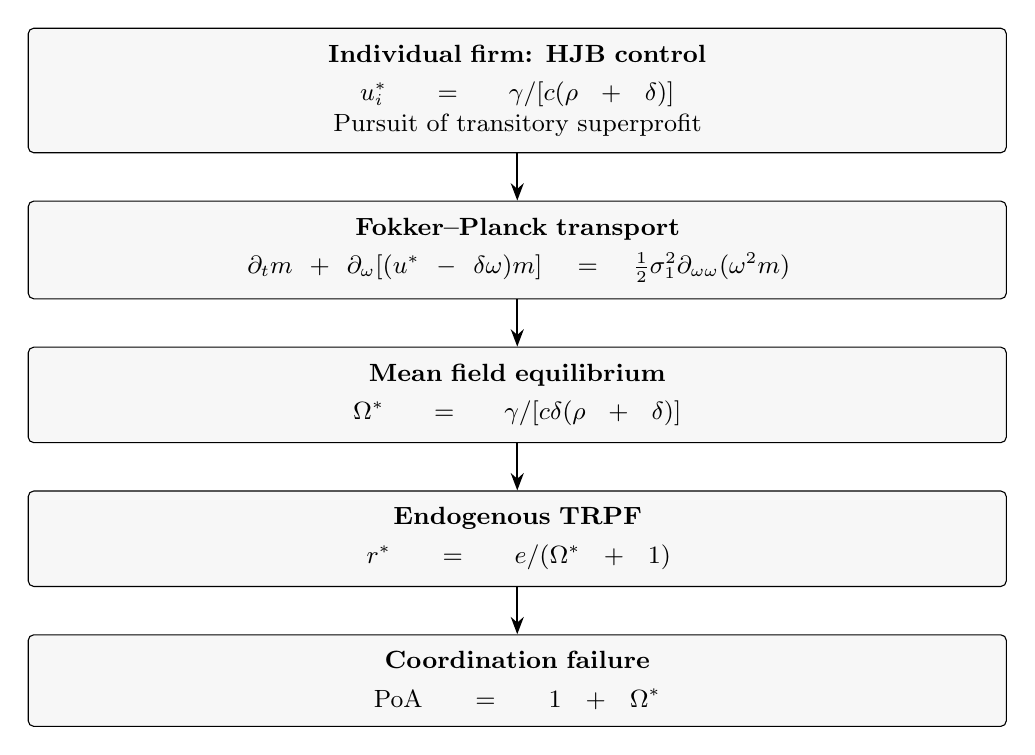
\begin{tikzpicture}[node distance=6mm]
\node[flowbox] (n0) {\textbf{Individual firm: HJB control}\\[3pt]$u_i^*=\gamma/[c(\rho+\delta)]$\\Pursuit of transitory superprofit};
\node[flowbox,below=of n0] (n1) {\textbf{Fokker--Planck transport}\\[3pt]$\partial_t m+\partial_\omega[(u^*-\delta\omega)m]=\frac12\sigma_1^2\partial_{\omega\omega}(\omega^2m)$};
\draw[flowarrow] (n0) -- (n1);
\node[flowbox,below=of n1] (n2) {\textbf{Mean field equilibrium}\\[3pt]$\Omega^*=\gamma/[c\delta(\rho+\delta)]$};
\draw[flowarrow] (n1) -- (n2);
\node[flowbox,below=of n2] (n3) {\textbf{Endogenous TRPF}\\[3pt]$r^*=e/(\Omega^*+1)$};
\draw[flowarrow] (n2) -- (n3);
\node[flowbox,below=of n3] (n4) {\textbf{Coordination failure}\\[3pt]$\mathrm{PoA}=1+\Omega^*$};
\draw[flowarrow] (n3) -- (n4);
\end{tikzpicture}
\caption{Trilogy architecture, Article 1: the real accumulation engine.}
\end{figure}

\begin{figure}[H]\centering
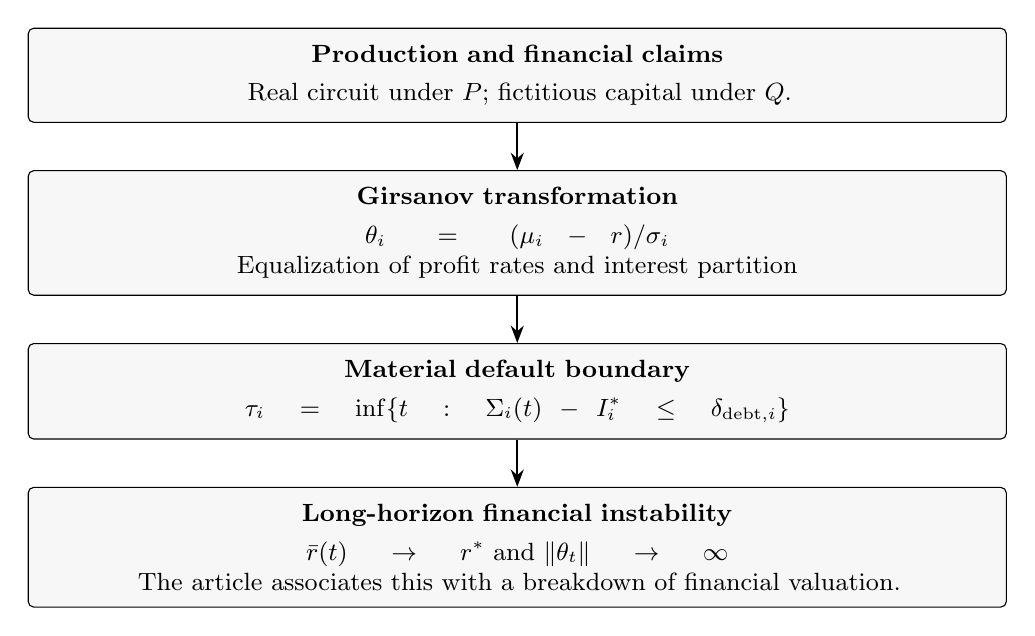
\begin{tikzpicture}[node distance=6mm]
\node[flowbox] (n0) {\textbf{Production and financial claims}\\[3pt]Real circuit under $P$; fictitious capital under $Q$.};
\node[flowbox,below=of n0] (n1) {\textbf{Girsanov transformation}\\[3pt]$\theta_i=(\mu_i-r)/\sigma_i$\\Equalization of profit rates and interest partition};
\draw[flowarrow] (n0) -- (n1);
\node[flowbox,below=of n1] (n2) {\textbf{Material default boundary}\\[3pt]$\tau_i=\inf\{t:\Sigma_i(t)-I_i^*\leq\delta_{\mathrm{debt},i}\}$};
\draw[flowarrow] (n1) -- (n2);
\node[flowbox,below=of n2] (n3) {\textbf{Long-horizon financial instability}\\[3pt]$\bar r(t)\to r^*$ and $\lVert\theta_t\rVert\to\infty$\\The article associates this with a breakdown of financial valuation.};
\draw[flowarrow] (n2) -- (n3);
\end{tikzpicture}
\caption{Trilogy architecture, Article 2: fictitious capital and measure change.}
\end{figure}

\begin{figure}[H]\centering
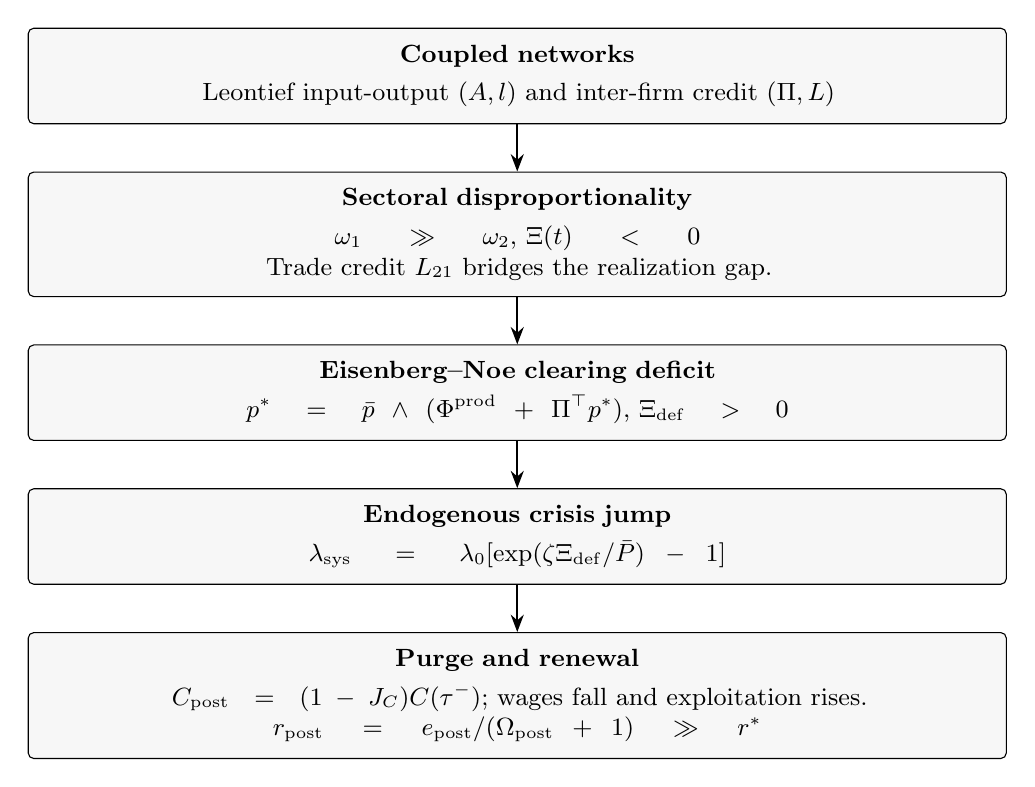
\begin{tikzpicture}[node distance=6mm]
\node[flowbox] (n0) {\textbf{Coupled networks}\\[3pt]Leontief input-output $(A,l)$ and inter-firm credit $(\Pi,L)$};
\node[flowbox,below=of n0] (n1) {\textbf{Sectoral disproportionality}\\[3pt]$\omega_1\gg\omega_2$, $\Xi(t)<0$\\Trade credit $L_{21}$ bridges the realization gap.};
\draw[flowarrow] (n0) -- (n1);
\node[flowbox,below=of n1] (n2) {\textbf{Eisenberg--Noe clearing deficit}\\[3pt]$p^*=\bar p\wedge(\Phi^{\mathrm{prod}}+\Pi^\top p^*)$, $\Xi_{\mathrm{def}}>0$};
\draw[flowarrow] (n1) -- (n2);
\node[flowbox,below=of n2] (n3) {\textbf{Endogenous crisis jump}\\[3pt]$\lambda_{\mathrm{sys}}=\lambda_0[\exp(\zeta\Xi_{\mathrm{def}}/\bar P)-1]$};
\draw[flowarrow] (n2) -- (n3);
\node[flowbox,below=of n3] (n4) {\textbf{Purge and renewal}\\[3pt]$C_{\mathrm{post}}=(1-J_C)C(\tau^-)$; wages fall and exploitation rises.\\$r_{\mathrm{post}}=e_{\mathrm{post}}/(\Omega_{\mathrm{post}}+1)\gg r^*$};
\draw[flowarrow] (n3) -- (n4);
\end{tikzpicture}
\caption{Trilogy architecture, Article 3: contagion, devalorization, and renewal.}
\end{figure}
\subsection{Structural Mapping: Neoclassical vs. Marxian Mathematical Finance}
\begingroup\small\begin{longtable}{|>{\raggedright\arraybackslash}p{0.20\textwidth}|>{\raggedright\arraybackslash}p{0.34\textwidth}|>{\raggedright\arraybackslash}p{0.34\textwidth}|}\hline
Foundational Concept & Neoclassical / Orthodox Mathematical Finance & Marxian Mathematical Finance (Trilogy Formulation) \\ \hline
\textbf{Origin of Value} & Subjective utility, marginal productivity, state-contingent claims. & Socially Necessary Labor Time (SNLT) converted via the MELT (${m}_{t}$). \\ \hline
\textbf{Risk-Neutral Measure ($Q$)} & An analytical pricing artifact resulting from absence of arbitrage (NFLVR). & The formal mathematical dual of the \textbf{equalization of profit rates} and capital fetishism ($M \dots M'$). \\ \hline
\textbf{Market Price of Risk ($\theta$)} & An exogenous subjective risk-aversion parameter. & The normalized deviation of branch valorization from the social average rate of profit: $\fitmath{{\theta }_{i}=\frac{1}{{\sigma }_{i}}\left({\frac{e}{{\gamma }_{i}+1}-\bar{r}}\right)}$. \\ \hline
\textbf{Asset Price Determination} & Discounted expected future cash flows ${E}^{Q}[\int{e}^{-rt}C{F}_{t}dt]$. & Capitalized legal claims on future surplus-value (\textbf{fictitious capital}), structurally bounded by living labor extraction: $\int{\delta }_{i}\leq \Sigma$. \\ \hline
\textbf{Corporate Default Barrier} & Exogenous asset-to-debt threshold (Merton structural equity barrier: ${V}_{t}\leq D$). & \textbf{Material valorization barrier:} When extracted surplus minus defensive automation capex fails to cover contractual debt service: ${\Sigma }_{i}-{I}_{i}^{*}\leq {\delta }_{i}$. \\ \hline
\textbf{Technical Change} & Exogenous Total Factor Productivity (TFP) shocks. & Endogenous \textbf{Mean Field Game arms race} where individual pursuit of superprofits ($\gamma$) drives systemic organic composition saturation (${\Omega }^{*}$). \\ \hline
\textbf{Market Inefficiency} & Market frictions, asymmetric information, behavioral biases. & \textbf{Price of Anarchy of Market Competition:} $PoA=1+{\Omega }^{*}$; the structural contradiction between individual rationality and systemic profit sustainability. \\ \hline
\textbf{Systemic Crises} & Exogenous tail risk, bank runs, liquidity freezes. & \textbf{Endogenous devalorization jumps} triggered when physical disproportionality (${\omega }_{1}\gg {\omega }_{2}$) breaks the Eisenberg-Noe debt-clearing lattice. \\ \hline
\textbf{Function of Crisis} & Inefficient market failure requiring monetary/fiscal stabilization. & \textbf{Organic cleansing mechanism:} Violent destruction of constant capital and expansion of the reserve army to reset $\Omega$ and restore the profit rate. \\ \hline
\end{longtable}\endgroup
\subsection{Epistemological Manifesto: Beyond Financial Fetishism}
This trilogy establishes three foundational theses for a critical mathematical finance:

\subsubsection{Thesis I: Mathematical Finance Must Abandon Capital Fetishism}
In standard mathematical finance, capital is written as a number in a differential equation that generates yields through the operator ${e}^{rt}$. This is the purest formalization of what Marx termed \textbf{commodity and capital fetishism}: the social relation of production between workers and capital appears as an autonomous, self-expanding property of money.

By grounding asset drift in the Monetary Expression of Labor Time (${m}_{t}$), the organic composition (${\omega }_{t}$), and the rate of exploitation (${e}_{t}$), mathematical finance restores the living worker to the center of asset valuation. Fictitious capital cannot self-expand; it merely discounts claims on surplus labor extracted at the point of production.

\subsubsection{Thesis II: The First Fundamental Theorem of Asset Pricing is Inherently Transitory}
Orthodox asset pricing assumes that an equivalent martingale measure $Q\sim P$ exists globally in time.

We have proved that under competitive accumulation, the TRPF forces the Girsanov kernel to diverge over long horizons:

\[\fitmath{\lim_{t \to \infty} \Vert{}\theta_t\Vert{} = \infty \implies \mathbb{E}^\mathbb{P}\left[ \exp\left( \frac{1}{2}\int_0^T \Vert{}\theta_t\Vert{}^2 dt \right) \right] = \infty}\]
The equivalent martingale measure $Q$ is not an eternal property of financial markets; it is an \textbf{ideological and mathematical construct that breaks down during valorization crises}. Financial derivatives and credit claims cannot be continuously hedged or priced as martingales when debt service outstrips the physical extraction of surplus-value.

\subsubsection{Thesis III: Crises Are Topological Necessities of Capitalist Reproduction}
Crises cannot be legislated away by macro-prudential capital requirements or central bank liquidity injections.

Because the microeconomic control problem of the firm forces every enterprise to automate to capture superprofits (${u}_{i}^{*}>0$), capitalist competition inexorably drives the macroeconomy toward over-accumulation (${\Omega }^{*}$). The resulting disproportionality between the means of production and the consumption fund inevitably ruptures the inter-firm credit clearing network ($\Pi$).

A financial crash is therefore the only mathematical operator capable of resolving the contradiction: it destroys constant capital through moral depreciation (${J}_{C}$), cancels uncollectible debt through repudiation (${J}_{F}$), and crushes wages via the reserve army of labor, resetting the organic composition and allowing the cycle of accumulation to resume.

\subsection{The Complete Trilogy Overview}
\begin{itemize}
\item \textbf{Article 1:} \emph{Microeconomic Foundations of the TRPF: Stochastic Automation, Superprofits, and Mean Field Equilibria}
\item \textbf{Article 2:} \emph{Fictitious Capital, Measure Changes, and Structural Credit Risk under the TRPF}
\item \textbf{Article 3:} \emph{Networked Valorization Crises: Inter-Departmental Credit Contagion and the Topology of Capitalist Devalorization}
\end{itemize}
This concludes the formal development of the three articles.

\end{document}
